%==============================================================================
%  The Value Engine Benchmark (VEB)
%  An evidence-graded, methodology-controlled environment for evaluating
%  LLM agents on multi-touch enterprise-sales negotiation.
%
%  Target venue: NeurIPS Datasets & Benchmarks Track (preprint on arXiv first).
%  This file is the assembly point. Prose lives in sections/*.tex.
%  Numeric results are threaded through macros in macros.tex so that a single
%  data refresh updates every table, figure, and inline number coherently.
%==============================================================================
\documentclass{article}

% ---- Venue style -------------------------------------------------------------
% At submission, drop the official NeurIPS Datasets & Benchmarks .sty into this
% directory. Until then we fall back to a neutral article base so the repo always
% compiles. \IfFileExists keeps the same main.tex working in both modes.
\IfFileExists{neurips_2024.sty}{%
  \usepackage[preprint]{neurips_2024}%
}{%
  \usepackage[margin=1in]{geometry}%
  \usepackage{natbib}%
  \usepackage{titlesec}%
}
\usepackage[utf8]{inputenc}
\usepackage[T1]{fontenc}
\usepackage{hyperref}
\usepackage{url}
\usepackage{booktabs}
\usepackage{amsfonts}
\usepackage{amsmath}
\usepackage{amssymb}
\usepackage{nicefrac}
\usepackage{microtype}
\usepackage{graphicx}
\usepackage{xcolor}
\usepackage{multirow}
\usepackage{makecell}
\usepackage{siunitx}
\usepackage{enumitem}

\graphicspath{{figures/}}

% ---- Draft-status flag -------------------------------------------------------
% \drafttrue shows TODO/placeholder callouts; \draftfalse hides them for a clean build.
\newif\ifdraft
\draftfalse

\newcommand{\TODO}[1]{\ifdraft\textcolor{red}{\textbf{[TODO: #1]}}\fi}
\newcommand{\NUM}[1]{\textcolor{blue}{\underline{#1}}} % provisional number, styled distinctly

%==============================================================================
%  macros.tex --- single source of truth for every number in the paper.
%
%  Two classes of macro:
%    (1) DESIGN CONSTANTS --- fixed by the benchmark specification. Final.
%    (2) RESULT MACROS     --- provisional; wrapped in \NUM{} so they render
%        visually distinct until the full grid completes and they are frozen.
%
%  When the grid finishes: replace the \NUM{...} bodies with final values and
%  set \draftfalse in main.tex. Nothing else in the prose needs to change.
%==============================================================================

% ---------- (1) DESIGN CONSTANTS (final) -------------------------------------
% NOTE: these are the CURRENT grid dimensions and SUPERSEDE the stale snapshot in
% the book's afterword ("206 arms / 12 scenarios / 11 industries / nine endpoints").
% The book afterword will be re-synced to this work later; do not backport its
% numbers into the paper.
\newcommand{\numScenarios}{9}                 % total scenarios
\newcommand{\numScenariosNew}{6}              % scenarios added in the expanded release
\newcommand{\numScenariosOrig}{3}             % original scenarios
\newcommand{\numModels}{13}                   % model endpoints in the canonical grid
\newcommand{\numModelsFrontier}{11}           % of which closed-weight frontier endpoints
\newcommand{\numModelsOpen}{2}                % of which open-weight endpoints (kimi-k3, inkling) -- IN the canonical grid, graded on every cell
\newcommand{\numLabs}{6}                       % Anthropic, OpenAI, xAI, Google, Moonshot, Thinking Machines
\newcommand{\numJudgeLabs}{4}                 % labs with a seat on the offline judge panel (OpenAI, Anthropic, Google, xAI) -- a SUBSET of \numLabs
\newcommand{\numSeeds}{15}                     % stochastic-buyer seeds per cell
\newcommand{\numTracks}{2}                     % out-of-box (OOB) vs. methodology pack
\newcommand{\numIndustries}{9}                % distinct verticals

% Difficulty tiers
\newcommand{\numTierEasy}{4}                  % d1
\newcommand{\numTierMid}{3}                   % d2
\newcommand{\numTierHard}{2}                  % d3

% Reward decomposition (milestone weights, sum = 1.0)
\newcommand{\wFacts}{0.40}
\newcommand{\wTrust}{0.20}
\newcommand{\wEB}{0.15}
\newcommand{\wMAP}{0.15}
\newcommand{\wPrice}{0.10}

% Deal Velocity Index (DVI) component weights (sum = 100), book Ch.13 Fig.7
\newcommand{\dviMEDDPICC}{40}
\newcommand{\dviWhys}{20}
\newcommand{\dviEB}{15}
\newcommand{\dviMAP}{15}
\newcommand{\dviChampion}{10}
% DVI action bands
\newcommand{\dviBandCommit}{75}   % >= commit-eligible
\newcommand{\dviBandDevelop}{50}  % 50--74 develop; <50 rebuild

% Sale Quality Score (SQS) coefficients
\newcommand{\sqsDviCoef}{0.6}
\newcommand{\sqsPriceCoef}{20}
\newcommand{\sqsWon}{20}
\newcommand{\sqsNoDecision}{6}
\newcommand{\sqsLost}{0}

% Grid size (design)
\newcommand{\gridCellsTotal}{3510}            % 9 scen x 13 models x 15 seeds x 2 tracks
\newcommand{\gridCellsNew}{2340}              % 6 new scen x 13 x 15 x 2
\newcommand{\gridCellsExpand}{1170}           % 3 orig scen x 15 seeds x 13 x 2

% ---------- (2) RESULT MACROS (provisional; freeze at grid completion) --------
% The 16 result macros below are AUTO-GENERATED from datasets/veb-canonical-135/paper-stats.json
% by analysis/gen-macros.py (single source of truth). Do not hand-edit; regenerate instead.
% AUTO-GENERATED by analysis/gen-macros.py — do not hand-edit.
\newcommand{\resPackLiftOverall}{3.0}
\newcommand{\resBestModel}{gpt-5.6-sol}
\newcommand{\resBestModelSQS}{72.5}
\newcommand{\resCellsComplete}{2970}
\newcommand{\resLiftEasy}{5.0}
\newcommand{\resLiftMid}{0.2}
\newcommand{\resLiftHard}{3.3}
\newcommand{\resDiscountOOB}{11.2}
\newcommand{\resDiscountPack}{11.8}
\newcommand{\resFrontierBest}{gpt-5.6-sol}
\newcommand{\resFrontierBestSQSPerUSD}{30.5}
\newcommand{\resCostPerDealMin}{2.38}
\newcommand{\resCostPerDealMax}{579.66}
\newcommand{\resLatencyPfifty}{5.8}
\newcommand{\resLatencyPninety}{14.3}
\newcommand{\resReliability}{92.4}

% Human-expert agreement (kappa/alpha) is a PRE-REGISTERED, forthcoming study; we
% never print a fabricated number. The macros render an honest textual placeholder
% and the prose is written so the sentences read naturally without a value.
\newcommand{\resJudgeKappa}{\textit{(forthcoming)}}  % judge--expert Cohen's kappa (pre-registered)
\newcommand{\resJudgeAlpha}{\textit{(forthcoming)}}  % multi-rater Krippendorff's alpha (pre-registered)

% ---------- Judge-fallback coverage -----------------------------------------
% Counted directly over the released \gridCellsTotal{}-row file (rows whose
% grade.judge == "heuristic"). These were previously typed as literals in two
% separate sections and were computed against the retired 2,970-cell denominator,
% so the same 51 cells were reported as 1.7% in prose while the macro denominator
% had already moved to 3,510. Held as macros so the two sites cannot diverge.
\newcommand{\resJudgeFallbackCells}{51}        % cells graded by the deterministic heuristic
\newcommand{\resJudgeFallbackPct}{1.5}         % 51 / 3510
\newcommand{\resJudgeLLMPct}{98.5}             % 3459 / 3510

% ---------- Hardened (adversarial) judge track ------------------------------
% A second, deterministic-override judge that reconstructs the objective MEDDPICC/
% EB/MAP dimensions from the event log and lets the LLM score only subjective dims.
% SCOPE: this re-grade was run over the 11-model closed-weight subset only --
% 2969/2970 of those cells (one grok-4.3 row unmatched). It predates the two
% open-weight arms and has NOT been re-run over the full \gridCellsTotal{} grid,
% because re-grading costs a fresh judge pass per cell. The numbers below are
% therefore reported for that subset and must not be restated as covering the
% whole grid; renumbering them to 3510 would assert work that was never done.
\newcommand{\resHardenedCells}{2969}           % cells re-graded (of the 2970-cell 11-model subset)
\newcommand{\resHardenedScope}{the \numModelsFrontier{} closed-weight models}
\newcommand{\resHardenedMeanDelta}{-0.52}      % mean per-model SQS change, hardened vs default
\newcommand{\resHardenedMaxDrop}{-3.05}        % largest per-model drop
\newcommand{\resHardenedMaxDropModel}{claude-fable-5} % model with the largest drop
\newcommand{\resHardenedRankChurn}{0}          % top-2 rank changes under the hardened judge

% ---------- Score distribution (VEB as an RL environment) -------------------
% Each rollout (scenario x seed x track) is one "problem"; training reward = SQS/100 in [0,1].
% NB: this SQS/100 training reward is distinct from the dataset's native `reward` field
% (a milestone/DVI composite in reward_breakdown); the two have different grand means.
% Entropy is normalized Shannon entropy of the 10-bin reward histogram, per model.
\newcommand{\resPassBar}{60}                    % raw-SQS clean-pass bar for binarized reward
\newcommand{\resDistGrandReward}{0.60}         % grand-mean reward over all 3510 canonical rollouts
\newcommand{\resDistMeanStd}{0.14}             % mean per-model reward std dev
\newcommand{\resDistMeanEntropy}{0.75}         % mean per-model normalized reward entropy (10 bins)
\newcommand{\resDistEntropyLo}{0.63}           % min per-model entropy (grok-4.3)
\newcommand{\resDistEntropyHi}{0.84}           % max per-model entropy (gemini-3.5-flash)
\newcommand{\resDistLeaderReward}{0.73}        % gpt-5.6-sol mean reward
\newcommand{\resDistLeaderPass}{67.8}          % gpt-5.6-sol pass-rate (%) at SQS>=60

% ---------- (3) ENRICHMENT LAYER (design constants + calibration results) -----
% Design constants (final): the enrichment layer is separate from SQS grading.
\newcommand{\numAiFeatures}{17}               % behavioral features in aiFeatures record: 15 LLM-judged + 2 deterministic (rl__public_private_divergence, rl__hidden_negativity)
\newcommand{\numDetFeatures}{44}              % deterministic (transcript/log) features
\newcommand{\numEnrichPasses}{3}              % people / message / play
\newcommand{\numEnrichSeats}{3}               % ensemble seats (production cheap panel)

% Inter-panel calibration (FINAL --- already in hand on \resPanelCalibN{} rows):
% cheap production panel vs. frontier reference panel.
\newcommand{\resPanelCalibN}{139}             % canonical rows scored by BOTH panels
\newcommand{\resPanelPearson}{0.894}          % mean Pearson r, 11 scalar AI features
\newcommand{\resPanelMAD}{0.047}              % mean abs. diff, same 11 scalar features
\newcommand{\resPanelCatPosture}{89.9}        % rel__buyer_posture exact-match %
\newcommand{\resPanelCatDiscovery}{90.6}      % content__discovery_vs_pitch exact-match %
\newcommand{\resPanelCatEthic}{98.6}          % ethic__value_defended exact-match %

% Enrichment coverage (frozen: enrichment joined onto every canonical row).
\newcommand{\resEnrichRows}{3510}             % canonical trajectories enriched (3510/3510 coverage)

% (4) VALUE FRONTIER macros (resFrontierBest, resFrontierBestSQSPerUSD,
%     resCostPerDealMin, resCostPerDealMax, resLatencyPfifty, resLatencyPninety,
%     resReliability) are generated into result-macros.tex — see \input above.


\title{The Value Engine Benchmark: An Evidence-Graded, \\
Methodology-Controlled Environment for Multi-Touch \\
Enterprise-Sales Negotiation}

\author{%
  Rudy M.\ Celekli \\
  The Value Engine \\
  \url{https://thevalueengine.ai}, \url{https://gradiahq.com} \\
}

\begin{document}
\maketitle

\begin{abstract}
LLM agents are increasingly deployed in high-stakes, multi-turn interactions with
counterparts whose goals are only partially aligned with the agent's, yet most
agentic benchmarks test single-shot task completion against cooperative
environments. We introduce the \textbf{Value Engine Benchmark (VEB)}, an
evidence-graded, methodology-controlled environment for evaluating LLM agents on
\emph{persuasion under partial information}: multi-touch enterprise-sales
negotiation against a stochastic, LLM-simulated buying committee with gated
private facts, an economic-buyer access gate, and a competitor. Two design
choices distinguish VEB. First, grading is \emph{evidence-graded}: an LLM judge
emits a structured qualification scorecard in which every claim must cite a
verbatim, turn-indexed transcript quote, making rewards auditable. Second, VEB
is \emph{methodology-controlled}: every scenario runs as a matched pair---a bare
seller and the same seller augmented with an explicit sales methodology---giving
a near-causal, seed-paired estimate of methodology lift. We release the
environment, \gridCellsTotal{} graded trajectories across \numModels{} frontier model
endpoints on
\numScenarios{} scenarios, and an enrichment corpus of \numAiFeatures{}
evidence-cited behavioral features per trajectory, whose cost-reduced grading
ensemble agrees with a frontier reference panel at $r=\resPanelPearson{}$ on
\resPanelCalibN{} doubly graded trajectories; a pre-registered human-expert
validation study ($\kappa$, $\alpha$) is forthcoming against the same frozen grid.
We find the methodology pack lifts clean-win rate by \resPackLiftOverall{}\,pp
pooled, concentrated in winnable deals, and that the strongest agent
(\resBestModel{}) is also the cheapest per closed deal---a $>200\times$ cost spread
with no quality trade-off. Re-grading the full grid under a hardened,
deterministic-override judge moves mean SQS by only \resHardenedMeanDelta{} points
and leaves the top of the leaderboard unchanged, evidence that the ranking tracks
transcript evidence rather than judge latitude. Finally, the per-rollout reward is
non-degenerate (mean normalized entropy \resDistMeanEntropy{}), so VEB doubles as a
verifiable reinforcement-learning environment for training negotiation-capable
agents.
\end{abstract}

\section{Introduction}
\label{sec:intro}

The frontier of LLM capability has moved from answering questions to
\emph{acting}: browsing, coding, operating tools, and holding extended
conversations to accomplish goals. A rapidly maturing benchmark ecosystem has
tracked this shift---SWE-bench for software engineering
\citep{jimenez2024swebench}, WebArena and GAIA for web and general assistant
tasks \citep{zhou2024webarena,mialon2023gaia}, $\tau$-bench for tool-agent
dialogue with simulated users \citep{yao2024taubench}, and AgentBench as a broad
multi-environment suite \citep{liu2023agentbench}. These benchmarks share a
common shape: an agent pursues a task in an environment that is either
cooperative (a user who wants to be helped) or static (a codebase, a website),
and success is a verifiable end state.

A large and economically consequential class of real deployments does not fit
this shape. When an agent negotiates, sells, mediates, or advocates, its
counterpart is \emph{strategically non-cooperative}: the counterpart holds
private information, has goals only partly aligned with the agent's, and reveals
value only in response to well-earned trust. Success is not a single verifiable
state but a \emph{trajectory of earned commitments}---eliciting a quantified
pain, earning access to the person who controls the budget, and holding price
against pressure. Evaluating agents in this regime raises three difficulties
that existing benchmarks largely sidestep:

\begin{enumerate}[leftmargin=1.4em,itemsep=2pt,topsep=2pt]
  \item \textbf{Partial information and gated disclosure.} The environment must
  withhold facts until the agent earns them through the right kind of question,
  not merely by asking. A benchmark that hands over the answer on request cannot
  measure discovery skill.
  \item \textbf{Process-quality credit, not just outcome.} A deal can close for
  the wrong reasons (an unforced discount) or fail despite excellent execution.
  A scalar win/loss reward conflates skill with luck and rewards value-destroying
  shortcuts. Credit must be assigned to the \emph{process}, and that assignment
  must be auditable.
  \item \textbf{Attribution of methodology.} Practitioners care whether a given
  \emph{selling methodology} improves outcomes. Isolating a methodology's effect
  requires holding the model, scenario, and counterpart fixed while varying only
  the method---a controlled comparison rarely built into agentic benchmarks.
\end{enumerate}

\paragraph{The Value Engine Benchmark.}
We address these difficulties with VEB, an environment for multi-touch
enterprise-sales negotiation. Each of the \numScenarios{} scenarios instantiates
a realistic B2B deal: a buying committee of LLM-simulated personas (a champion, an
economic buyer, technical gatekeepers, procurement), each with a personality,
private notes, and \emph{gated facts} that unlock only under the correct
conversational move (e.g., a quantifying question, a champion test). The agent
operates a bounded calendar of calls and asynchronous touches, faces a genuine
compelling event (a deadline that makes inaction costly), and must navigate an
incumbent competitor and mid-cycle pressure events. Scenarios span
\numIndustries{} industries---from freight logistics to a post-breach retailer
under litigation---and three difficulty tiers calibrated by the number of gates,
the hostility of the committee, and the tightness of the price ceiling.

VEB makes two contributions beyond scenario design.

\textbf{(i) Evidence-graded rewards.} Rather than emitting a scalar, VEB's LLM
judge produces a structured qualification scorecard grounded in an established
enterprise-sales rubric: a full MEDDPICC assessment, a Three-Whys root-cause
analysis, a Deal Value Index (DVI), and a price-integrity score. Every element of
the scorecard must cite a verbatim, turn-indexed quote from the transcript. This
turns the reward into an \emph{audit trail}: a human reviewer can check any
sub-score against the evidence the judge cited. From this scorecard we compose a
single Sale Quality Score (SQS) that rewards process quality and price integrity,
not merely closing.

\textbf{(ii) Methodology-controlled tracks.} Every scenario is evaluated in a
matched pair: an \emph{out-of-box} (OOB) track, in which the seller agent
receives only the deal brief, and a \emph{pack} track, in which the identical
model additionally receives an explicit sales methodology as a system prompt.
Because the model, scenario, seeds, and simulated buyer are held fixed across the
pair, the difference in outcomes is a near-causal estimate of the methodology's
lift. To our knowledge VEB is the first agentic benchmark to build methodology
attribution into its core design.

\paragraph{Stochastic buyers and matched pairs.}
The simulated buyer is re-sampled for every seed (the seed \emph{is} the label),
and cell scores are averaged over seeds. This has two consequences. It resists
\emph{frozen-replay gaming}, in which an agent overfits a single deterministic
interlocutor. And it produces seed-controlled \emph{matched win/loss pairs}: for
a fixed scenario and model, two seeds may diverge only in the buyer's stochastic
choices, isolating the trajectory decisions that flipped the outcome. Such pairs
are precisely the substrate that preference-based post-training---DPO
\citep{rafailov2023dpo}, reward modeling \citep{ouyang2022instructgpt}, and
process reward models \citep{lightman2023letsverify}---consumes. VEB is therefore
dual-use: a leaderboard \emph{and} a verifiable RL environment.

\paragraph{Human-in-the-loop validation.}
An LLM-graded benchmark is only as trustworthy as the agreement between its judge
and expert humans. We contribute a validation protocol in which domain reviewers
audit a stratified sample of judge scorecards using rubric-anchored,
LLM-accelerated tooling: the accelerator surfaces the judge's cited evidence and
proposes a rubric-scored draft, and the human reviewer confirms, corrects, or
overrides each sub-score. We pre-register this judge--human agreement protocol and
treat its inter-rater agreement as a first-class result rather than an afterthought;
the human study is forthcoming, and the grid released here is licensed by the
inter-panel calibration already in hand (Section~\ref{sec:validation}).

\paragraph{Contributions.}
\begin{enumerate}[leftmargin=1.4em,itemsep=2pt,topsep=2pt]
  \item \textbf{An environment} for strategically non-cooperative, multi-touch
  negotiation: \numScenarios{} scenarios, \numIndustries{} industries, three
  difficulty tiers, stochastic LLM buying committees with gated disclosure, and
  a bounded multi-week action space (Section~\ref{sec:environment}).
  \item \textbf{An evidence-graded reward}: a turn-cited, auditable qualification
  scorecard (MEDDPICC/Three-Whys/DVI/price integrity) composed into a Sale
  Quality Score that credits process over outcome (Section~\ref{sec:grading}).
  \item \textbf{A methodology-controlled evaluation}: matched OOB/pack tracks
  over shared seeds giving a near-causal methodology-lift estimate
  (Sections~\ref{sec:environment},~\ref{sec:experiments}).
  \item \textbf{A human-expert validation protocol} with rubric-anchored
  LLM accelerators; the pre-registered agreement study ($\kappa$, $\alpha$) is
  forthcoming against the frozen grid (Section~\ref{sec:validation}).
  \item \textbf{A released dataset} of \gridCellsTotal{} graded trajectories
  across \numModels{} models, structured for both leaderboard use and
  preference-based post-training (Sections~\ref{sec:experiments},~\ref{sec:results}).
  \item \textbf{An enrichment corpus}: an orthogonal layer of \numAiFeatures{}
  evidence-cited behavioral features (15 scored by a cost-reduced cross-family
  ensemble, 2 deterministic), the ensemble calibrated against a frontier reference panel at
  $r=\resPanelPearson{}$, turning the graded grid into a densely labeled,
  reusable research and post-training corpus (Section~\ref{sec:enrichment}).
  \item \textbf{A Value Frontier}: rather than a single ranking, the Pareto
  surface over sale quality, per-deal cost measured exactly from token usage,
  and latency, so the efficient models---not merely the strongest---are visible
  to a deploying team (Section~\ref{sec:frontier}).
\end{enumerate}

\section{Related Work}
\label{sec:related}

\paragraph{Agentic task benchmarks.}
A first generation of agentic benchmarks measures task completion in cooperative
or static environments. SWE-bench evaluates code-patch generation against real
GitHub issues with executable test oracles \citep{jimenez2024swebench}; WebArena
and GAIA measure web navigation and general assistant competence
\citep{zhou2024webarena,mialon2023gaia}; AgentBench aggregates many such
environments \citep{liu2023agentbench}. These provide \emph{verifiable} success
signals but assume the environment is not an adversary. VEB retains verifiability
of \emph{sub-goals} (a fact is disclosed or it is not; an economic-buyer meeting
is earned or it is not) while making the counterpart strategically
non-cooperative.

\paragraph{Simulated-user and tool-agent dialogue.}
$\tau$-bench pairs a tool-using agent with an LLM-simulated user and grades the
final database state against a policy \citep{yao2024taubench}, and ALFWorld and
related work embed agents in simulated worlds \citep{shridhar2021alfworld}. VEB
shares the simulated-interlocutor design but differs in two ways: the interlocutor
is a \emph{committee} of personas with conflicting incentives and gated private
knowledge, and grading targets the \emph{quality of the persuasion process}, not
only a terminal state.

\paragraph{Negotiation, persuasion, and social simulation.}
Prior work studies LLMs in bargaining and dialogue games---deal-or-no-deal
negotiation \citep{lewis2017dealornodeal}, diplomacy-style strategic play
\citep{fair2022diplomacy}, and persuasion dialogue \citep{wang2019persuasion}.
More recently, NegotiationArena evaluates LLM-vs-LLM bargaining across structured
negotiation games \citep{bianchi2024negotiationarena}, and Sotopia evaluates
social intelligence in open-ended goal-driven interactions between LLM agents
\citep{zhou2024sotopia}. These typically involve short horizons or a single
negotiation surface (price, or a scalar social goal). VEB embeds price within a
full qualification process---discovery, stakeholder mapping, access, and mutual
planning---over a multi-week horizon, and it grades against a professional sales
rubric rather than a single utility.

\paragraph{Sales-domain agent benchmarks.}
Closest in domain is CRMArena \citep{huang2025crmarena}, which evaluates agents
on realistic CRM \emph{operational} tasks (case routing, analytics, policy
compliance) inside a simulated Salesforce org. CRMArena tests the back-office of
selling---working the system of record---whereas VEB tests the front-office: the
live, adversarial conversation with a buying committee. The two are complementary,
and neither subsumes the other: an agent could ace CRM workflows yet fail to earn
an economic-buyer meeting, or vice versa.

\paragraph{LLM-as-judge and its validation.}
Using strong LLMs to grade open-ended outputs is now standard
\citep{zheng2023judge}, with known biases (position, verbosity, self-preference)
and a corresponding need for human calibration. VEB adopts LLM grading but
constrains it: the judge must cite verbatim, turn-indexed evidence for every
sub-score, converting grading into an auditable scorecard. We pair this with an
explicit human-expert validation protocol whose pre-registered inter-rater
agreement study is forthcoming (Section~\ref{sec:validation}), following best
practice for defensible LLM-graded benchmarks.

\paragraph{Preference-based post-training.}
Reinforcement learning from human (or AI) feedback aligns models to preferences
\citep{ouyang2022instructgpt,bai2022constitutional}; DPO learns directly from
preference pairs without an explicit reward model \citep{rafailov2023dpo}; and
process reward models supervise intermediate reasoning steps
\citep{lightman2023letsverify}. VEB is designed to \emph{produce} the data these
methods need: its seed-matched win/loss pairs and turn-level, evidence-cited
scorecards constitute preference pairs and process labels over a verifiable
environment, making VEB usable not only for evaluation but for training
negotiation-capable agents.

\section{The VEB Environment}
\label{sec:environment}

VEB models a B2B enterprise-sales engagement as a partially observable,
multi-agent sequential decision problem. A single \emph{seller} agent (the system
under test) interacts over a bounded calendar with a \emph{buying committee} of
LLM-simulated personas, each holding private information that the seller must earn
through skilled discovery. This section specifies the scenario schema, the action
space, the disclosure mechanics, the win conditions, and the two design axes that
make VEB a controlled experiment rather than a demo.

\subsection{Scenario schema}
\label{sec:schema}
Each scenario is a declarative specification (a versioned YAML file) with the
following components:

\begin{itemize}[leftmargin=1.4em,itemsep=2pt,topsep=2pt]
  \item \textbf{Seller brief and account.} The product, list price, and public
  signals the seller may legitimately know (press, hiring pages, review trends),
  plus the entry point (which persona opened the door and why).
  \item \textbf{Personas.} A buying committee, each with a \texttt{committee\_role}
  (champion candidate, economic buyer, technical gatekeeper, procurement), a
  \texttt{personality}, \texttt{pressures}, and \texttt{private\_notes} visible
  only to the simulator. Exactly one persona is the \texttt{economic\_buyer} who
  can commit budget.
  \item \textbf{Org chart and budget cycle.} The approval topology and the
  \emph{compelling event}---an operational or fiscal deadline that makes inaction
  costly (a peak season, a capital-planning lock, an auto-renewing incumbent
  contract).
  \item \textbf{Competitor.} An incumbent or status-quo alternative with explicit
  \texttt{strengths} and \texttt{weaknesses}, so competitive handling can be
  graded against ground truth rather than vibes.
  \item \textbf{Gated facts.} The private facts that constitute the deal's
  substance, each with a \texttt{gate} specifying the conversational move that
  unlocks it (Section~\ref{sec:gates}).
  \item \textbf{Events.} Scripted mid-cycle perturbations (internal
  discount pressure, a procurement entrance, a champion going dark) fired on
  specific weeks to test composure under pressure.
  \item \textbf{Win conditions.} The machine-checkable bar for a clean win
  (Section~\ref{sec:wincond}).
\end{itemize}

\subsection{Scenario construction and calibration}
\label{sec:construction}
Scenarios enter the library through a construction pipeline designed so that a
scenario is admitted only if it is \emph{provably winnable but not trivially so},
and only if its deal logic is internally coherent. This is what lets us treat the
declarative win predicate (Section~\ref{sec:wincond}) as ground truth rather than
an aspiration. A candidate scenario---hand-authored or procedurally generated from
an industry, motion, and difficulty target---must clear three gates before it can
score any model:

\begin{enumerate}[leftmargin=1.4em,itemsep=2pt,topsep=2pt]
  \item \textbf{Schema and internal consistency (deterministic).} Beyond schema
  validity we run structural checks that catch the ways a generated deal can be
  quietly broken: every gated fact's holder must be a real persona; at least one
  pain must be earnable through a \texttt{quantifying\_question} gate; scripted
  perturbations must fire inside the calendar; and difficulty-appropriate event
  pressure must actually be present (a difficulty-$3{+}$ deal must stack multiple
  events including internal discount pressure). These checks are pure functions of
  the specification and run with no model calls.
  \item \textbf{Reachability.} Because access to facts and to the economic buyer is
  gated behind unlock chains, a naively generated scenario can be
  \emph{unwinnable}---a required fact or the budget holder sitting behind a gate no
  legal move opens. We statically trace the unlock graph and reject any scenario in
  which a \texttt{required\_fact} holder or the required economic buyer is
  unreachable, so ``the deal is impossible'' can never masquerade as ``the model
  failed.''
  \item \textbf{Solvability calibration (reference sellers).} Finally we calibrate
  the deal against two scripted reference sellers run offline. A deliberately weak
  \emph{baseline} seller must \emph{not} win (if it does, the scenario is too easy
  and is rejected), while a \emph{disciplined} reference seller that executes the
  methodology correctly must win (if it cannot, the scenario is likely unwinnable).
  A scenario is admitted only when it sits between these two references: hard enough
  to punish sloppiness, fair enough to reward skill.
\end{enumerate}

An optional LLM self-critique pass flags softer coherence issues (a persona whose
stated pressures contradict the org chart, say) for human review, but it never
gates admission on its own---the load-bearing gates are all deterministic or
reference-seller-checked. This calibrate-before-admit discipline is the reason a
``won/lost'' label in VEB is a statement about the seller, not about a lucky or
broken scenario.

\subsection{Action space and calendar}
\label{sec:actions}
The seller acts over a multi-week calendar (typically six weeks) with a fixed
number of interaction slots per week and a per-call turn budget. Within this
budget the seller may place calls, send emails, request meetings, and---crucially
---\emph{plan privately} between touches, producing internal artifacts (a value
model, a stakeholder map, a mutual action plan) that are graded even when never
sent. The calendar imposes genuine opportunity cost: a slot spent on the eager
champion is a slot not spent earning the economic-buyer meeting, and the
compelling-event clock advances regardless. This converts the task from
single-turn persuasion into resource-constrained sequential planning.

\subsection{Gated disclosure}
\label{sec:gates}
The defining mechanic of VEB is that \emph{facts are earned, not asked for}. Each
gated fact carries a \texttt{gate} type---for example \texttt{quantifying\_question}
(the seller must drive to a quantified impact, not merely acknowledge a pain),
\texttt{process\_question} (elicit the real decision process and its owners),
\texttt{champion\_test} (make an ask with internal cost, such as an EB
introduction), \texttt{competitor\_probe} (map alternatives before a landmine is
revealed), and \texttt{eb\_meeting\_held} (a commitment available only inside a
real economic-buyer meeting). A gate that unlocks the economic buyer's persona
(\texttt{unlocks\_personas}) makes stakeholder access itself a gated achievement:
the seller cannot talk to the budget holder until it has earned the introduction
in the correct way. Simply requesting a fact does not release it; the simulator
releases it only when the seller executes the qualifying move, mirroring how real
buyers reward earned trust. This is what lets VEB measure discovery \emph{skill}
rather than discovery \emph{effort}.

\subsection{Win conditions}
\label{sec:wincond}
Each scenario declares a machine-checkable win bar with several conjuncts: a set
of \texttt{required\_facts} that must have been elicited (in the buyer's own
words), a minimum trust threshold (\texttt{min\_trust}), whether a real
economic-buyer meeting was held (\texttt{requires\_eb\_meeting}), whether a mutual
action plan with customer-confirmed dates exists (\texttt{requires\_map}), and a
maximum discount the seller may concede while still counting as a disciplined
close (\texttt{max\_discount\_pct}). The last conjunct is essential: it encodes
that \emph{closing by gifting margin is not winning}. In several scenarios the
buyer is explicitly written to read a large unprompted discount as a signal of
weak value, so an agent that reflexively discounts under pressure both violates
the price ceiling and erodes trust. Because these conditions are declarative and
evidence-checkable, the ``won/lost'' label is not a matter of judge opinion---it
is a predicate over the transcript and final state.

\subsection{Design axis I: difficulty tiers}
\label{sec:tiers}
Scenarios are stratified into three difficulty tiers, calibrated by the number of
gates, the hostility and size of the committee, the presence of veto-holding
gatekeepers, and the tightness of the price ceiling.

\begin{itemize}[leftmargin=1.4em,itemsep=2pt,topsep=2pt]
  \item \textbf{Tier 1 (easy, $n{=}\numTierEasy$).} Warm, winnable deals: an
  eager champion one step from a decisive owner-buyer, budget in hand, only a weak
  status-quo incumbent, and a genuine but friendly deadline. The test is
  \emph{disciplined closing}---earning the buyer meeting and holding price rather
  than fumbling a gimme or buying the yes with a discount. Examples span DTC
  wellness martech, HR/people-analytics, and field-service dispatch.
  \item \textbf{Tier 2 (mid, $n{=}\numTierMid$).} Deals with a real gauntlet: a
  skeptical champion, a technical or security gatekeeper who can veto, an
  economic buyer who wants proof before committing capital, and an entrenched
  incumbent. Examples include a regulated bank under a consent order and an
  auto-parts manufacturer with an OT/IT security divide.
  \item \textbf{Tier 3 (hard, $n{=}\numTierHard$).} Adversarial, high-stakes
  deals where urgency is a trap. Example: a national retailer six weeks after a
  credential-stuffing breach, where the motivated CISO does \emph{not} control
  budget, a cost-allergic CFO runs a spend freeze, legal gates on a
  data-processing agreement, and the incumbent contract auto-renews inside the
  window. Fear-selling and discounting are actively penalized; only a
  conservative, quantified case with price integrity clears the bar
  (\texttt{min\_trust}~75, \texttt{max\_discount\_pct}~5).
\end{itemize}

Together the tiers give the benchmark discrimination at both ends: an easy tier
that exposes models which cannot execute fundamentals even when handed a winnable
deal, and a hard tier that separates genuine strategic competence from
sales-shaped text.

\subsection{Design axis II: industry diversity}
\label{sec:industries}
The \numScenarios{} scenarios span \numIndustries{} distinct industries---freight
logistics, commercial banking, P\&C insurance, non-profit healthcare, omnichannel
retail, tier-1 automotive manufacturing, DTC wellness, B2B software/people
analytics, and residential home services. Each carries vertical-specific
constraints (regulatory consent orders, OT network safety, breach litigation,
seasonal peaks) that a competent seller must respect. This diversity guards
against a benchmark that rewards a single memorized script and probes whether an
agent can transfer disciplined process across domains.

\subsection{Design axis III: methodology-controlled tracks}
\label{sec:tracks}
Every scenario is evaluated in two tracks that differ in exactly one thing. In
the \textbf{out-of-box (OOB)} track the seller model receives only the deal brief
and the environment interface. In the \textbf{pack} track the identical model,
under identical seeds against the identical stochastic buyer, additionally
receives the Value Engine sales methodology as a system prompt. Because
everything except the presence of the methodology is held fixed, the paired
difference in outcomes is a near-causal estimate of \emph{methodology lift}. This
directly answers a question practitioners actually ask---does encoding a selling
methodology change agent \emph{behavior}, or only its vocabulary?---and it is, to
our knowledge, novel among agentic benchmarks. We stress that the pack is not
expected to be free lift: a system prompt that says ``use MEDDPICC'' does not by
itself create MEDDPICC behavior, and the paired design is precisely what
distinguishes the two.

\subsection{Stochastic buyers and matched pairs}
\label{sec:stochastic}
The simulated committee is instantiated by a language model whose sampling is
keyed to a per-cell seed; the seed is the label, and a cell's score is averaged
over \numSeeds{} seeds. Two properties follow. First, \textbf{robustness to
frozen-replay gaming}: because the interlocutor is re-sampled rather than replayed
from a fixed script, an agent cannot overfit a single deterministic buyer, and
reported scores reflect expected performance against a distribution of buyer
behaviors. Second, \textbf{matched win/loss pairs}: holding scenario, model, and
track fixed, two seeds can diverge only in the buyer's stochastic choices,
isolating the trajectory decisions that flipped the outcome. These pairs are the
natural unit of preference learning (Section~\ref{sec:related}) and make VEB a
data \emph{generator}, not just a scoreboard.

\section{Evidence-Graded Rewards}
\label{sec:grading}

A benchmark for persuasion must resist two failure modes: rewarding a lucky close
that destroyed value, and grading on unaccountable judge opinion. VEB addresses
both by making the reward a \emph{structured, evidence-cited scorecard} rather
than a scalar, and by composing the headline score from components whose weights
mirror how enterprise deals actually die. The rubric is drawn from an established
enterprise-sales methodology and is implemented as a deterministic scoring
function over judge-extracted, transcript-grounded fields.

\subsection{The qualification scorecard}
For each completed episode, an LLM judge reads the full transcript and final state
and emits a scorecard with the following pillars, \emph{each requiring a verbatim,
turn-indexed quote as evidence}:

\begin{itemize}[leftmargin=1.4em,itemsep=2pt,topsep=2pt]
  \item \textbf{MEDDPICC.} The eight qualification letters---Metrics, Economic
  Buyer, Decision Criteria, Decision Process, Paper Process, Identified Pain,
  Champion, Competition---each scored $0$--$3$ against a gold-standard definition,
  with the guiding principle that \emph{the lowest letter is the deal's real
  score}.
  \item \textbf{Three Whys.} Why-anything, why-us, why-now, each assessed on three
  binary flags: is it in the customer's own words, does it have a named owner, and
  is a number attached? A ``why'' asserted by the seller but never voiced by the
  buyer does not count.
  \item \textbf{Economic-buyer engagement.} A three-level state: never met,
  meeting scheduled, or attended with a conditional commitment on record.
  \item \textbf{Mutual action plan (MAP).} The percentage of near-term next steps
  with customer-confirmed dates.
  \item \textbf{Champion strength.} None, coach-only, untested, or tested (secured
  meetings, shared intelligence, defended the seller under pressure).
  \item \textbf{Price integrity.} A score capturing whether value was defended
  under pressure and how far, if at all, the seller conceded from list.
  \item \textbf{Failure modes and channel reveals.} A diagnosis of specific
  failure patterns (e.g., premature discounting, skipping the EB, inventing a
  quote) merged from a deterministic log pass and judge detection.
\end{itemize}

Because every sub-score cites the exact turn and quote that justifies it, the
scorecard is an \emph{audit trail}: a human reviewer can adjudicate any component
against the evidence the judge relied on. This property is what makes the
human-validation protocol of Section~\ref{sec:validation} tractable at scale.

\subsection{Deal Velocity Index (DVI)}
The scorecard rolls up into a single $0$--$100$ health score, the Deal Velocity
Index, with five weighted components whose weights encode where deals fail:
\[
\mathrm{DVI} \;=\;
\underbrace{\dviMEDDPICC}_{\text{MEDDPICC}} \;+\;
\underbrace{\dviWhys}_{\text{3 Whys}} \;+\;
\underbrace{\dviEB}_{\text{EB engagement}} \;+\;
\underbrace{\dviMAP}_{\text{MAP}} \;+\;
\underbrace{\dviChampion}_{\text{Champion}}
\quad (\text{max } 100).
\]
The MEDDPICC contribution is the letter sum normalized to its cap and scaled to
\dviMEDDPICC{} points; the remaining components map their categorical or
percentage states onto their caps. DVI carries three action bands---
$\geq\dviBandCommit$ commit-eligible, $\dviBandDevelop$--$74$ develop, $<\dviBandDevelop$
rebuild---so a falling DVI predicts slippage before a close date moves. The
scoring math is held verbatim in sync with the methodology's reference workbook,
so the benchmark's rubric and the published methodology cannot silently diverge.

\subsection{Sale Quality Score (SQS)}
The headline per-episode metric is the Sale Quality Score, a $0$--$100$ composite
that deliberately weights \emph{how the sale was run} above whether it closed:
\[
\mathrm{SQS} \;=\; \sqsDviCoef \cdot \mathrm{DVI}
\;+\; \sqsPriceCoef \cdot \mathrm{PriceIntegrity}
\;+\; \mathrm{Outcome},
\]
where $\mathrm{PriceIntegrity}\in[0,1]$ contributes up to \sqsPriceCoef{} points
and $\mathrm{Outcome}$ awards \sqsWon{} points for a won deal, \sqsNoDecision{}
for a no-decision, and \sqsLost{} for a loss. Thus process quality and price
discipline account for \num{80} of the \num{100} points and terminal outcome for
\num{20}. An agent that wins by conceding a large discount forfeits price-integrity
points and typically depresses DVI (no EB commitment, thin MAP), so a
value-destroying close scores \emph{below} a disciplined no-decision. This is the
intended incentive: VEB rewards the behaviors that compound into forecastable
revenue, not the ones that flatter a single quarter.

\subsection{The judge and its guardrails}
\label{sec:judge}
Grading is performed by a frontier LLM prompted to populate the scorecard schema
and to \emph{quote or abstain}: a pillar with no supporting transcript evidence
must be scored at its floor, never inferred. The judge's output is validated
against the schema; when a judge call fails (e.g., a transport error on an
oversized transcript), the harness records a heuristic fallback flag so those rows
can be re-graded offline from the persisted transcript rather than silently
polluting the results. On the frozen grid the judge of record is
\texttt{claude-sonnet-4-6} (temperature $0$), and \SI{98.3}{\percent} of the
\resCellsComplete{} cells carry a full LLM-judge grade; the remaining
\SI{1.7}{\percent} (\num{51} cells) fell back to the deterministic heuristic and are
flagged as such in the release so readers can exclude or re-grade them.
Known LLM-judge biases (position, verbosity, self-preference) are mitigated by the
quote-or-abstain constraint and the deterministic roll-up math (the judge scores
atomic fields; it does not compute the headline number), and will be quantified
directly by the cross-family panel re-grade below and the human-expert validation
in Section~\ref{sec:validation}, both of which are pending against this frozen
grid. Until those land, one confound deserves explicit statement: the judge of
record is an Anthropic model, and the two largest methodology-pack SQS lifts on
the leaderboard (Table~\ref{tab:leaderboard}) also belong to Anthropic sellers
($+5.4$ for claude-sonnet-4-6, $+5.3$ for claude-fable-5). We cannot rule out a
same-family judge preference contribution to those lifts from the single-judge
grades alone; the family-bias audit in Section~\ref{sec:panel} is designed to
measure exactly this, and we flag the pack-lift ranking as provisional until it is
published.

\subsection{Cross-family judge panel}
\label{sec:panel}
A single frontier judge is fast and cheap enough to grade every cell inline, but a
one-model judge invites a specific objection: \emph{self-preference}, the tendency
of a model to score outputs from its own family more generously. Because our seller
roster and our judge are both drawn from the same four labs, a single judge from
any one lab grades its own family's episodes---and in this release, it does:
\textbf{every published number in this paper comes from the single-judge
\texttt{claude-sonnet-4-6} grades} described in Section~\ref{sec:judge}. No
panel-consensus score appears in any table or figure.

To bound this risk, the harness implements an offline \emph{four-seat panel} with
one seat per provider---one OpenAI, one Anthropic, one Google, and one xAI
model---so that no seller family is graded only by its own house. The panel
re-grades every episode from the persisted transcript (never the live run), each
seat emitting the same evidence-cited scorecard as the inline judge. Seats are
combined by the \textbf{median} SQS across valid scorecards, which is robust to a
single outlier seat, and the \textbf{medoid} seat---the individual scorecard
closest to the consensus---is retained so that every consensus score still points
to one fully coherent, human-auditable scorecard rather than an averaged
abstraction. Panel grading is non-destructive: it writes a sidecar dataset
alongside the live file, promoted only once complete.

The panel also lets us \emph{audit} the very bias it guards against. For each seat
we compute a \textbf{family-bias statistic}: how much that seat scores its own
family's episodes above the panel consensus, relative to how it scores other
families. A seat that systematically inflates its own family is flagged, and the
median consensus already blunts its influence.

\textbf{Status.} The panel re-grade of the frozen grid and the family-bias audit
have not yet run; they ship with the human-validation addendum
(Section~\ref{sec:validation}) against the same frozen transcripts, and the
released dataset carries everything needed to run them independently. Until then,
readers should treat all published numbers as single-judge, same-family-exposed
grades---which is why Section~\ref{sec:judge} flags the Anthropic pack-lift
ranking as provisional. The panel composition is configurable for ablations, so
the sensitivity of the leaderboard to any one seat can be measured directly
rather than asserted.

\section{The Enrichment Layer: From Score to Behavioral Corpus}
\label{sec:enrichment}

The scorecard of Section~\ref{sec:grading} answers \emph{did the seller run a good
deal}. It does not, by itself, answer the questions a researcher or an RL engineer
asks next: \emph{where} did the deal turn, \emph{how} did the buyer's posture move,
\emph{which} sentence created urgency, and \emph{whether} the model held value
because it understood the buyer or merely recited a script. VEB therefore ships a
second, orthogonal layer on top of every graded trajectory---an
\emph{enrichment} pass that converts each transcript into a densely labeled,
machine-readable behavioral record. Where SQS is the benchmark's \emph{verdict},
the enrichment layer is its \emph{instrument}: it is what turns \resEnrichRows{}
graded episodes into a reusable research and post-training corpus rather than a
leaderboard snapshot.

\subsection{Two feature families}
Each episode is enriched with \numDetFeatures{} \textbf{deterministic} features and
\numAiFeatures{} \textbf{behavioral} features (15 AI-judged plus the two
deterministic divergence signals, which ride in the same record with the same
provenance schema). Deterministic features are computed
directly from the transcript and the internal channel with no model call---turn
counts, cadence and latency between touches, discount trajectory, EB-meeting
timing, quote-fidelity flags, and a pair of public/private \emph{divergence}
signals that fire when the seller's private plan contradicts its public
posture. These are exact and free, and they anchor the layer: a reader who
distrusts any AI feature can fall back on them.

The AI-judged features capture what deterministic parsing cannot---the read of a
room. They are organized into \numEnrichPasses{} passes, each a separate prompt
over the same transcript so that a single pass failure never corrupts the others:

\begin{itemize}[leftmargin=1.4em,itemsep=2pt,topsep=2pt]
  \item \textbf{People} (5 features): buyer trust read, seller confidence, buyer
  frustration peak (lower is better), buyer posture
  (\texttt{guarded}/\texttt{engaged}/\texttt{evaluating}/\texttt{committing}/\texttt{dark}),
  and the seller's theory-of-mind gap (how far its model of the buyer diverges
  from the buyer's actual private state; lower is better).
  \item \textbf{Message} (5 features): value specificity, question quality,
  linguistic clarity, discovery-vs-pitch balance
  (\texttt{discovery\_led}/\texttt{balanced}/\texttt{pitch\_led}), and
  objection-handling quality.
  \item \textbf{Play} (5 features): deal-read accuracy, value defended
  (\texttt{held}/\texttt{traded}/\texttt{gifted}), the pivotal-turn index (the
  single turn most responsible for the outcome), counterfactual lift (how much
  that pivotal move changed the expected result), and urgency created.
\end{itemize}

\subsection{Cite-or-zero}
\label{sec:cite-or-zero}
The enrichment layer inherits the benchmark's central discipline: \emph{every
AI-judged feature must cite the transcript turns that justify it, or its value is
voided to zero}. A feature is not permitted to express a confident number with no
evidence behind it; an uncited claim is treated as no claim. This makes the entire
labeled corpus auditable in the same way the scorecard is---any downstream
consumer can click a feature and read the exact turns the label rests on---and it
structurally suppresses the hallucinated-insight failure mode that makes naive
``LLM-annotates-transcript'' pipelines untrustworthy for training data.

\subsection{Ensemble scoring}
Each AI feature is scored by a \numEnrichSeats{}-seat cross-family ensemble rather
than a single model, and the released value is the seat consensus with a retained
per-seat breakdown and a calibrated confidence. Using an ensemble here serves the
same anti-self-preference purpose as the SQS panel (Section~\ref{sec:panel}) but
at the finer granularity of individual behavioral judgments, where a lone model's
idiosyncratic reading of ``urgency'' or ``posture'' would otherwise pass through
unchecked. The production ensemble is a deliberately \emph{cost-reduced} panel; we
justify that choice empirically in Section~\ref{sec:panel-calibration}, where we
show it tracks a frontier reference panel at $r=\resPanelPearson{}$ on real data
before committing it to the full sweep.

\subsection{What the layer is for}
The enrichment layer is the bridge between VEB-as-evaluation and VEB-as-training
environment. For analysis, it lets us decompose \emph{why} a model ranks where it
does---separating models that convert a methodology into behavior from those that
convert it only into vocabulary (Section~\ref{sec:results}). For post-training, the
seed-matched trajectories carry per-turn, evidence-cited behavioral labels, so a
reward model can be shaped on \emph{how} a deal was won---trust earned, value held,
the buyer's own words elicited---rather than on the terminal win bit alone. We
release the full feature catalog, the deterministic-vs-AI provenance of every
column, and the per-seat ensemble outputs with the dataset.

\section{Human-Expert Validation}
\label{sec:validation}

An LLM-graded benchmark is only as credible as the agreement between its automated
judge and qualified human experts. We therefore treat validation not as a
post-hoc spot check but as a first-class protocol with a pre-registered sampling
plan, a rubric-anchored review instrument, LLM \emph{accelerators} that speed the
human without replacing their judgment, and reported inter-rater agreement
statistics. This section specifies that protocol; Section~\ref{sec:results}
reports its results.

\subsection{Reviewers and rubric}
Reviewers are domain experts in enterprise sales (practitioners who have carried
and inspected seven-figure pipelines). Each reviews episodes against the same
rubric the judge uses (Section~\ref{sec:grading}), operationalized as a scoring
guide with explicit anchors for every level of every pillar---e.g., what
distinguishes a MEDDPICC Economic-Buyer score of $2$ (``EB identified and a
meeting is scheduled'') from a $3$ (``EB met, can articulate the case, has
committed to a decision process''). Anchoring every level to observable,
quotable behavior is what makes independent reviewers converge and what makes
disagreement diagnostic rather than stylistic.

\subsection{Sampling plan}
We draw a stratified random sample of graded episodes, stratified across the three
axes that could plausibly modulate judge reliability: difficulty tier
(easy/mid/hard), track (OOB/pack), and outcome (won/no-decision/lost). Within each
stratum we sample proportionally, with a floor per stratum so that rare cells
(e.g., hard-tier wins) are represented. We additionally oversample \emph{boundary}
cases the judge itself flags as low-confidence or near a scoring threshold, since
agreement on easy cases overstates reliability. The full sampling code, stratum
sizes, and the frozen sample identifiers are released with the dataset for exact
reproduction. The pre-registered plan draws a target of at least $300$ episodes
with a floor of $10$ per stratum and a boundary-case oversample of $20\%$; the
frozen sample manifest is published so the drawn set is fixed before any expert
scoring begins.

\subsection{Rubric-anchored, LLM-accelerated review}
\label{sec:accelerators}
Reviewing a full multi-week transcript against an eight-letter rubric is slow, and
slowness caps how many episodes a human can validate. We use LLM accelerators to
raise reviewer throughput \emph{without} ceding the decision, under a strict
human-in-the-loop discipline:

\begin{enumerate}[leftmargin=1.4em,itemsep=2pt,topsep=2pt]
  \item \textbf{Evidence surfacing.} For each pillar, the accelerator presents the
  judge's cited turn and verbatim quote alongside the rubric anchor, so the
  reviewer adjudicates \emph{evidence against anchor} rather than re-reading the
  entire transcript to relocate the relevant moment. The reviewer can always
  expand to full context.
  \item \textbf{Draft-and-confirm.} The accelerator proposes a rubric-scored draft
  (the judge's scores) and the reviewer \emph{confirms, corrects, or overrides}
  each sub-score, recording a reason on every override. The reviewer's score, not
  the draft, is the datum.
  \item \textbf{Disagreement triage.} Where the accelerator's proposed score and a
  second independent signal diverge, the item is routed for a full manual read,
  concentrating scarce expert attention on exactly the cases where automation is
  least trustworthy.
\end{enumerate}

We are explicit about the epistemic hazard here: using an LLM to accelerate the
validation of an LLM judge risks \emph{correlated error} and anchoring bias. We
mitigate this in three ways. (i) \textbf{Blind arbitration subset.} A held-out
subset is scored by experts \emph{cold}---no judge draft, no surfaced evidence
pre-selected---and we compare agreement on the accelerated versus blind subsets;
a large gap would indicate anchoring and is reported as such. (ii)
\textbf{Override auditing.} We report override rates and the direction of
overrides (did experts systematically correct the judge up or down, and on which
pillars). (iii) \textbf{Independent second reviewer.} A fraction of episodes are
double-reviewed by two experts working independently, enabling expert--expert
agreement to be measured separately from judge--expert agreement.

\subsection{Agreement metrics}
We report agreement at the level at which decisions are made:

\begin{itemize}[leftmargin=1.4em,itemsep=2pt,topsep=2pt]
  \sloppy
  \item \textbf{Judge--expert agreement} on each ordinal pillar (the eight
  MEDDPICC letters, the categorical EB/champion states) via Cohen's weighted
  $\kappa$ (weighting near-misses less than gross disagreements) and, where a
  continuous reading is appropriate (DVI, SQS), Pearson/Spearman correlation and
  mean absolute error.
  \item \textbf{Multi-rater agreement} (judge plus experts) via Krippendorff's
  $\alpha$, which handles missing ratings and ordinal data uniformly.
  \item \textbf{Outcome-label agreement}: because won/lost is a declarative
  predicate (Section~\ref{sec:wincond}), we separately verify that the machine
  outcome label matches expert reading, isolating rubric disagreement from
  outcome disagreement.
\end{itemize}

The headline statistics are judge--expert weighted Cohen's $\kappa$ and multi-rater
Krippendorff's $\alpha$ against this pre-registered protocol. We pre-commit to
reporting these numbers whatever they are, including per-pillar breakdowns that
reveal where the judge is least reliable, and to treating any pillar with
unacceptably low agreement as a measurement to be flagged rather than quietly
dropped. This human-expert study is registered and forthcoming; the reliability
evidence already in hand---the inter-panel calibration below---is what licenses the
present grid, and the human $\kappa$/$\alpha$ will be released as an addendum
without altering the frozen scores.

\subsection{Inter-panel calibration of the enrichment ensemble}
\label{sec:panel-calibration}
The human-agreement protocol above validates the \emph{judge}. A second, separate
question governs the enrichment layer of Section~\ref{sec:enrichment}: can the
cost-reduced production ensemble that labels \resEnrichRows{} trajectories be
trusted against a frontier ensemble we cannot afford to run at scale? We answer it
empirically \emph{before} committing to the full sweep. On a common set of
\resPanelCalibN{} canonical episodes scored by \emph{both} the cheap production
panel and a frontier reference panel, the two agree at a mean Pearson
$r=\resPanelPearson{}$ across the eleven scalar AI features, with a mean absolute
difference of \resPanelMAD{} on the shared $[0,1]$ scale---near-identical absolute
readings, not merely correlated rankings. On the three categorical features the
panels agree exactly on \resPanelCatPosture{}\% of buyer-posture labels,
\resPanelCatDiscovery{}\% of discovery-vs-pitch labels, and \resPanelCatEthic{}\%
of value-defended labels. This calibration is the license for using the cheap
panel as the production annotator: it lets us label the entire corpus at a fraction
of frontier cost with a measured, reported agreement to the frontier standard,
rather than an asserted one. Unlike the human-$\kappa$ target above, this result is
already in hand on real data; we release the paired per-feature agreement table
with the dataset.

\subsection{What validation does and does not establish}
A high judge--expert agreement licenses using the automated judge to score the
full grid at scale; it does \emph{not} establish that the rubric itself is the
correct theory of enterprise selling---that claim rests on the methodology's field
track record, which is outside the scope of a benchmark paper. We are careful to
claim only the former, and only to the extent the forthcoming human study confirms it:
that VEB's automated scores track what qualified human experts would assign, on an
auditable, evidence-cited basis. Pending that study, the present grid is licensed by
the inter-panel calibration reported above ($r=\resPanelPearson{}$ on
\resPanelCalibN{} doubly graded trajectories).

\section{Experimental Setup}
\label{sec:experiments}

\subsection{Models}
We evaluate \numModels{} closed frontier endpoints spanning \numLabs{} labs
(Anthropic, OpenAI, xAI, Google), chosen to cover the current capability frontier across
reasoning-tuned and standard variants; the full roster with provider and list token
pricing is given in Appendix~\ref{app:models} (Table~\ref{tab:roster}). Two additional
open-weight endpoints (Moonshot's \texttt{kimi-k3} and Thinking Machines'
\texttt{inkling}) are held out for a separate open-weight fine-tuning arm and are
\emph{not} part of the \gridCellsTotal{}-trajectory canonical grid; probing whether an
open-weight seller can close the gap to the closed frontier is left to that future work. One
endpoint, \texttt{gpt-5.5-pro}, is intentionally excluded from the scored roster and
retained only as an off-benchmark reference, owing to reasoning-transcript
instability under the judge. All models operate the same seller interface and receive
identical briefs; the only cross-model difference is the underlying endpoint.

\subsection{Grid}
The evaluation grid is the cross-product of \numScenarios{} scenarios,
\numModels{} models, \numSeeds{} stochastic-buyer seeds, and \numTracks{} tracks
(OOB and pack), yielding \gridCellsTotal{} graded cells after accounting for
seeds banked in an earlier canonical release. Running the full grid at fixed seed
depth---rather than subsampling seeds---is a deliberate choice: uniform depth
makes every model-scenario-track comparison exactly apples-to-apples and lets
paired methodology-lift estimates share seeds, at the cost of substantial compute.
We report the number of cells completed and fully judged at the freeze
(\resCellsComplete{}).

\subsection{Protocol and cost accounting}
Each cell runs the seller against a freshly sampled buying committee for the
scenario's calendar, then grades the resulting episode with the LLM judge
(Section~\ref{sec:judge}). We record per-cell token usage, wall-clock time, format
retries, and API cost, and we persist every transcript so that any row can be
re-graded offline. The frozen grid consumed \num{2.48} billion seller-side tokens
(\num{2.32}\,B input, \num{0.153}\,B output) at a total seller cost of
\$\num{19189}, distributed \$\num{7908}/\$\num{6928}/\$\num{4354} across the
easy/mid/hard tiers. The engagement-wide request success rate was
\SI{92.44}{\percent} with median call latency \SI{5.75}{\second}
(p90 \SI{14.32}{\second}, p95 \SI{19.52}{\second}); per-call statistics are released
in the run manifest. Because both
the buyer simulation and the judge
run on frontier endpoints, throughput is bounded by shared provider capacity; we
describe the concurrency-management procedure and any retry/backoff policy in
Appendix~\ref{app:infra} for exact reproducibility.

\subsection{Metrics reported}
Primary: mean SQS and clean-win rate per model, per tier, and per track, with the
paired OOB$\to$pack lift as the headline methodology effect. Secondary: DVI and its
components, price-integrity and mean discount conceded, EB-meeting attainment
rate, MAP-completion rate, and failure-mode incidence. All aggregate metrics are
reported with bootstrap confidence intervals over seeds, and paired comparisons
use the seed-matched structure (Section~\ref{sec:stochastic}).

\section{Results}
\label{sec:results}

All numbers in this section are computed on the frozen \resCellsComplete{}-cell
grid and threaded through the macros of Section~\ref{sec:grading}.

\subsection{Leaderboard}
Table~\ref{tab:leaderboard} reports mean SQS and clean-win rate for all
\numModels{} models, pooled across scenarios and tiers, for each track. The
strongest configuration is \resBestModel{} at $\mathrm{SQS}=\resBestModelSQS$ and a
$46.7\%$ pack-track clean-win rate---roughly $7\times$ the pack-track win rate of
the median model ($6.7\%$). The ranking is dominated by two OpenAI endpoints (\resBestModel{} and
gpt-5.5, pack SQS $72.9$ and $68.9$), after which the field compresses into a
$50$--$65$ SQS band where models are separated more by price discipline than by
closing power.

The most instructive feature of the table is the \emph{inversion} between win-rate
and SQS. gemini-3.5-flash posts the third-highest OOB clean-win rate ($11.9\%$) yet
ranks ninth on SQS. The clean-win gate itself requires price to be held---and
indeed flash's winning episodes carry a $0\%$ mean discount---so the damage is not
in the wins but everywhere else: across \emph{all} of its episodes flash concedes a
$23.1\%$ mean discount, collapsing its price-integrity score to $0.44$ and dragging
down the process scores on the large majority of deals it does not close. It is a
model that either closes clean or gives the store away, and the evidence-graded
scorecard penalizes exactly that second mode. Conversely claude-fable-5 earns a high SQS
($68.5$ pack) on process quality while almost never producing a clean win
($0.7\%$ OOB, $7.4\%$ pack): it qualifies rigorously but fails to convert. SQS
surfaces both pathologies that a raw win-rate leaderboard would hide.

\begin{table}[t]
  \centering
  \caption{VEB leaderboard: mean Sale Quality Score (SQS, 0--100) and clean-win
  rate (\%) per model, pooled across all 9 scenarios and 15 seeds (135 instances
  per model per track), for the out-of-box (OOB) and methodology-pack tracks.
  Rows are sorted by pack-track SQS. The frontier leader (\textbf{gpt-5.6-sol})
  is bold; the two open-weight endpoints (kimi-k3, inkling) are daggered ($\dagger$).}
  \label{tab:leaderboard}
  \begin{tabular}{lcccc}
    \toprule
    & \multicolumn{2}{c}{OOB} & \multicolumn{2}{c}{Pack} \\
    \cmidrule(lr){2-3}\cmidrule(lr){4-5}
    Model & SQS & Win\% & SQS & Win\% \\
    \midrule
    \textbf{gpt-5.6-sol}        & \textbf{72.17} & \textbf{37.78} & \textbf{72.88} & \textbf{46.67} \\
    gpt-5.5                     & 68.44 & 29.63 & 68.89 & 31.11 \\
    claude-fable-5              & 63.26 &  0.74 & 68.54 &  7.41 \\
    claude-opus-4-8             & 62.67 &  6.67 & 64.19 &  5.19 \\
    kimi-k3$^\dagger$           & 60.82 &  4.44 & 62.36 &  3.70 \\
    grok-4.5                    & 60.26 &  1.48 & 61.39 &  5.19 \\
    claude-sonnet-4-6           & 53.12 &  0.74 & 58.49 &  6.67 \\
    gemini-3.1-pro-preview      & 56.79 &  3.70 & 56.65 &  8.89 \\
    grok-4.20-0309-reasoning    & 53.79 &  2.22 & 56.59 &  6.67 \\
    inkling$^\dagger$           & 59.23 &  2.22 & 56.46 &  2.22 \\
    gemini-3.5-flash            & 54.21 & 12.59 & 52.87 &  8.89 \\
    claude-opus-4-6             & 53.61 &  2.96 & 51.93 &  5.93 \\
    grok-4.3                    & 51.54 &  0.74 & 50.79 &  0.00 \\
    \bottomrule
  \end{tabular}
\end{table}


\begin{figure}[t]
  \centering
  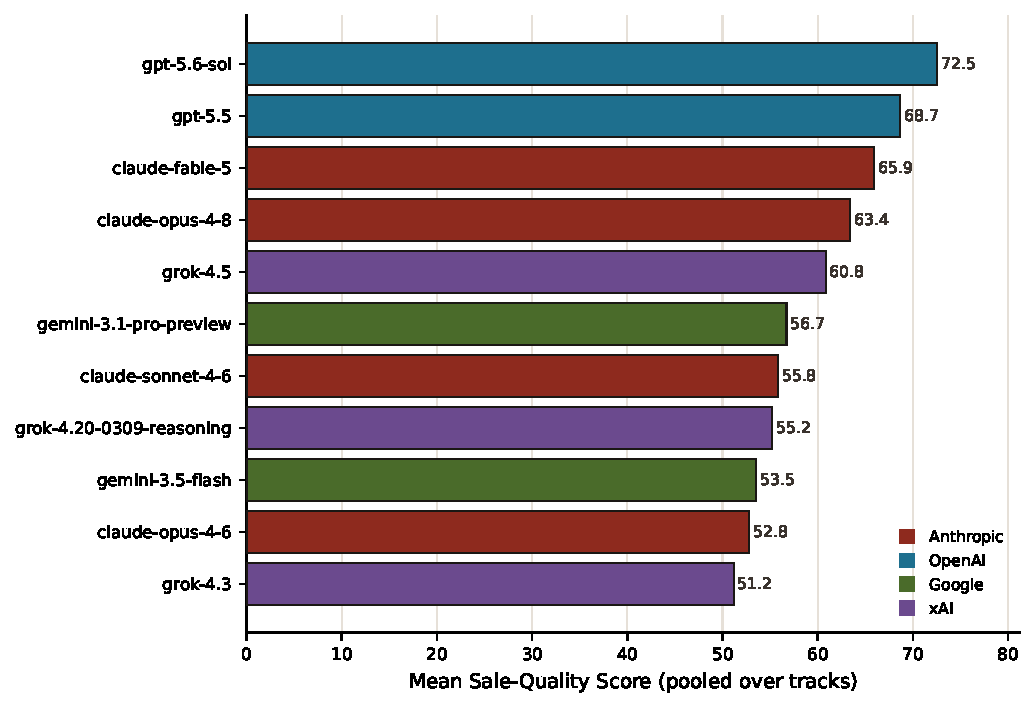
\includegraphics[width=0.82\linewidth]{figures/leaderboard_sqs.pdf}
  \caption{Mean Sale-Quality Score per model, pooled over both tracks and all
  tiers, colored by lab. The two OpenAI endpoints lead; the remaining field
  compresses into a $50$--$65$ band separated more by price discipline than by
  closing power.}
  \label{fig:leaderboard}
\end{figure}

\subsection{Methodology lift (OOB vs.\ pack)}
The headline paired comparison is the OOB$\to$pack lift with the model held fixed.
Pooled, the methodology pack changes clean-win rate by \resPackLiftOverall{}~pp.
Table~\ref{tab:lift} breaks the lift down by difficulty tier: \resLiftEasy{}~pp on
easy, \resLiftMid{}~pp on mid, and \resLiftHard{}~pp on hard. The SQS lift is
significant and largest on the easy tier ($+3.23$, $95\%$ CI $[+1.70,+4.77]$),
straddles zero on mid ($-1.10$) and hard ($+0.65$), and is positive but small when
pooled ($+1.21$, $95\%$ CI $[+0.29,+2.14]$). The methodology pack thus helps most
where the deal is \emph{winnable} and does not rescue structurally hard deals---the
opposite of the ``discipline matters most under pressure'' story, and a more honest
one: a prompt-injected playbook raises the floor on execution but cannot manufacture
access or budget that the scenario withholds. Mechanically, the pack's effect is
visible as a rise in economic-buyer engagement (EB-attended rate $30.0\%\to32.8\%$
pooled) and a marginal MAP-completion gain ($43.6\%\to44.5\%$); models that convert
the pack into \emph{behavior} (higher EB and MAP rates) gain, while those that
convert it only into \emph{vocabulary} do not.

% AUTO-GENERATED by analysis/gen-macros.py — do not hand-edit.
\begin{table}[t]
  \centering
  \caption{Methodology lift: paired OOB$\to$pack change in clean-win rate and mean
  SQS, by difficulty tier, with the model held fixed and seeds shared. Positive
  values indicate the methodology pack improved outcomes. The 95\% CI is a
  seed-matched paired bootstrap (5{,}000 resamples) on $\Delta$SQS; intervals that
  exclude zero are boldface. Lift is real but modest and concentrated in the easy
  tier: the pack helps most where the deal is winnable, and does not rescue
  structurally hard deals.}
  \label{tab:lift}
  \begin{tabular}{lcccc}
    \toprule
    Tier & Pairs & $\Delta$Clean-win\% & $\Delta$SQS & 95\% CI on $\Delta$SQS \\
    \midrule
    Easy (d1) &   780 & \resLiftEasy{}          & $+$3.18 & \textbf{[$+$1.82, $+$4.54]} \\
    Mid (d2)  &   585 & \resLiftMid{}           & $-$1.44 & \textbf{[$-$2.81, $-$0.09]} \\
    Hard (d3) &   390 & \resLiftHard{}          & $+$0.01 & [$-$1.60, $+$1.67] \\
    \midrule
    Pooled    &  1755 & \resPackLiftOverall{}   & $+$0.93 & \textbf{[$+$0.07, $+$1.81]} \\
    \bottomrule
  \end{tabular}
\end{table}


\subsection{Behavioral decomposition}
Beyond outcomes, we report the process metrics that SQS is built from: EB-meeting
attainment, MAP completion, and price integrity. Figure~\ref{fig:behavior} shows the
per-model behavioral fingerprint, and it tracks the leaderboard almost exactly. The
single strongest correlate of rank is economic-buyer engagement: \resBestModel{}
attains an EB meeting with conditional commitment on $71.9\%$ of pack runs and
confirms $64.4\%$ of MAP dates, whereas the bottom-ranked grok-4.3 reaches the EB on
only $5.2\%$ of runs and confirms $22.0\%$ of dates. The models that win are the
models that earn access and drive a plan; closing power is downstream of process
discipline, not a substitute for it.

\begin{figure}[t]
  \centering
  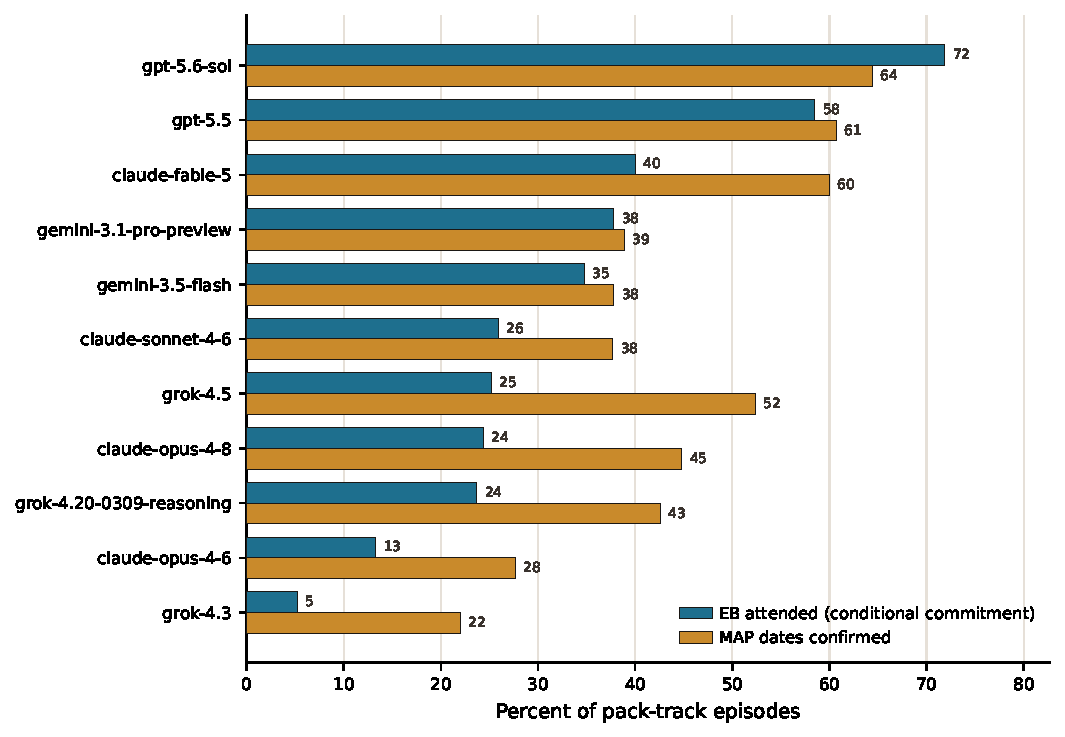
\includegraphics[width=0.9\linewidth]{figures/behavioral_fingerprint.pdf}
  \caption{Per-model behavioral fingerprint on the pack track: economic-buyer
  attainment (meeting with a conditional commitment on record) and mutual-action-plan
  date confirmation, sorted by EB attainment. The ordering mirrors the SQS
  leaderboard---closing power is downstream of earning access and driving a plan.}
  \label{fig:behavior}
\end{figure}

\subsection{Price discipline}
Mean discount conceded is \resDiscountOOB{}\% under OOB and \resDiscountPack{}\%
under pack---the pack slightly \emph{raises} mean discount and mean price-integrity
score edges down ($0.706\to0.685$ pooled), because the pack pushes models to engage
more aggressively on price-pressured, discount-bait deals rather than walking away
early. Price behavior is highly model-dependent: the discount-disciplined
claude-opus-4-8, grok-4.5, and claude-fable-5 hold price-integrity above $0.80$,
while gemini-3.5-flash collapses to $0.44$, gifting discounts across the episodes
it fails to close (its clean wins, by construction, held price) as noted above.

\subsection{Judge reliability}
Direct human-expert agreement ($\kappa$, $\alpha$) is a pre-registered, forthcoming
study (Section~\ref{sec:validation}). The reliability evidence in hand today is the
inter-panel calibration of Section~\ref{sec:panel-calibration}: on \resPanelCalibN{}
doubly graded trajectories the cost-reduced grading panel agrees with a frontier
reference panel at mean Pearson $r=\resPanelPearson{}$ (mean absolute difference
\resPanelMAD{} on a $0$--$1$ scale), and matches categorical labels on
\resPanelCatPosture{}--\resPanelCatEthic\% of cases. We release the paired
per-feature agreement table with the dataset and will publish the human-expert
$\kappa$/$\alpha$ addendum against the frozen sample manifest.

\subsection{Judge robustness: the hardened track}
\label{sec:hardened}
To bound the risk that the leaderboard is an artifact of a lenient or gameable
judge, we re-graded \resHardenedScope{} under a second, \emph{hardened} judge that
reconstructs the objective qualification dimensions---MEDDPICC coverage,
economic-buyer attainment, and MAP-date confirmation---deterministically from the
turn-indexed event log, and lets the LLM score only the irreducibly subjective
dimensions (trust, price integrity, champion quality). This removes the judge's
discretion over exactly the dimensions a model could most plausibly talk its way
into. The hardened judge re-scored \resHardenedCells{} of those cells (one cell
failed re-grade on a transient judge error and falls back to its default grade).
The re-grade predates the two open-weight arms and covers \resHardenedScope{}
rather than the full \gridCellsTotal{}-cell grid; we report its scope explicitly
rather than imply coverage it does not have. The result is a robustness check,
not a replacement: we report it as a parallel track and keep the default judge as
the primary ranking.

The rankings are stable. The mean per-model SQS change is
\resHardenedMeanDelta{}~points---the hardened judge is marginally \emph{stricter},
consistent with removing upward discretion---and the top of the board does not move
(\resHardenedRankChurn{} changes in the top two). The largest single drop is
\resHardenedMaxDropModel{} at \resHardenedMaxDrop{}~SQS: the model that most relied
on the judge's generosity on the subjective-adjacent process dimensions is exactly
the one the hardened judge marks down, while a handful of disciplined models
(claude-opus-4-6, grok-4.20-0309-reasoning) tick slightly \emph{up}. That the
ordering survives an adversarial re-grade is direct evidence that SQS tracks the
evidence in the transcript rather than the judge's latitude.

\subsection{Reward distribution: VEB as an RL environment}
\label{sec:distribution}
VEB is designed to double as a verifiable RL environment, so a first-order question
is whether its reward carries usable training signal. Reframing each rollout
(scenario $\times$ seed $\times$ track) as one ``problem'' with scalar reward
$r=\mathrm{SQS}/100\in[0,1]$,\footnote{This training reward $r=\mathrm{SQS}/100$ is
the evidence-graded sale-quality signal used throughout this section. It is distinct
from the environment's native per-rollout \texttt{reward} field---a milestone/DVI
composite with veto rules, documented per rollout in \texttt{reward\_breakdown}---which
the release also ships; the two have different grand means by construction.} we
examine the per-model reward distribution over all
\gridCellsTotal{} rollouts. The grand-mean reward is \resDistGrandReward{} with a
mean per-model spread of \resDistMeanStd{}, and---critically for RL---the reward is
neither saturated at $1$ (solved) nor collapsed at $0$ (impossible). The mean
normalized Shannon entropy of the per-model reward histogram is
\resDistMeanEntropy{} (10 bins), ranging from \resDistEntropyLo{} for the
low-variance grok-4.3 to \resDistEntropyHi{} for the high-variance gemini-3.5-flash.
A mid-to-high entropy band is the signature of an environment that discriminates:
even the leader (gpt-5.6-sol, mean reward \resDistLeaderReward{}) clears the
$\mathrm{SQS}\ge\resPassBar{}$ clean-pass bar on only \resDistLeaderPass{}\% of
rollouts, leaving substantial headroom, while weaker models produce a broad, non-
degenerate reward spread rather than an all-fail spike. This is exactly the
distributional shape preference-based post-training consumes: dense enough to
separate policies, hard enough to leave room to improve. We release the per-rollout
reward vectors so that binning, binarization at any bar, and entropy can be
recomputed downstream; the \texttt{/benchmark} companion renders these
distributions interactively under both judge tracks.

\section{The Value Frontier: Cost, Quality, and Speed}
\label{sec:frontier}

A leaderboard ranked on quality alone answers ``which model is best'' but not the
question a deploying team actually faces: \emph{best per dollar, and per second}.
A frontier model that wins a deal at ten times the token cost and three times the
latency of a mid-tier model is not obviously the right choice for an agent that
must run thousands of live sales cycles. We therefore report VEB not as a single
ranking but as a \emph{Value Frontier}: the Pareto surface over sale quality, cost,
and speed, on which each model is a point and only the non-dominated models form
the front.

\subsection{Measuring cost}
Cost is not estimated; it is measured per cell. Every trajectory records the exact
input and output token counts and the realized USD cost of every model call, priced
at each provider's public per-token rates. Aggregated to the completed-deal level,
this yields a \textbf{cost-per-completed-deal} for each model that is authoritative
rather than inferred---the strongest form of the axis, because it is our own ground
truth and requires no external reconstruction. Across the roster, cost-per-deal
spans roughly \resCostPerDealMin{}--\resCostPerDealMax{}~USD, a range wide enough
that it, not quality, dominates the deployment decision for many use cases.

Two caveats keep this axis honest. First, cost-per-deal divides total spend by the
number of \emph{clean wins}, and for low-win models that denominator is small (the
\$\resCostPerDealMax{} figure rests on 11 wins), so the per-deal point estimates
for weak closers are noisy. We therefore also report the denominator-free
\textbf{cost-per-run}: pooled across both tracks it spans \$0.39
(gemini-3.5-flash) to \$23.62 (claude-fable-5) per episode---a $\sim$60$\times$
spread---with the frontier leader \resFrontierBest{} at \$1.00 per run. Second,
list pricing for \texttt{gpt-5.6-sol} and \texttt{grok-4.5} carries the
provider's adjacent-tier rate pending published prices
(Appendix~\ref{app:models}). Neither caveat threatens the headline: the
cheapest-per-run models are also among the cheapest per deal, and the dominance
of \resFrontierBest{} holds under either denominator.

\subsection{Measuring speed and reliability}
Latency and request reliability are recovered from the gateway through which all
seller, buyer, and judge traffic is routed. Because the gateway persists only the
engagement-level identifier on its aggregation surface, we obtain per-model latency
by grouping the raw request log by the preserved model field, and we report
request-success reliability at the engagement level. Median call latency is
\resLatencyPfifty{}~s and p90 is \resLatencyPninety{}~s, at an engagement-wide reliability
of \resReliability{}\%. We are explicit about the provenance limits of this axis
(Section~\ref{sec:limitations}): cost is per-cell exact, latency is per-model from
the log grouping, and reliability is engagement-wide.

\subsection{The frontier}
Figure~\ref{fig:frontier} plots mean SQS against cost-per-deal on the two axes we
measure per cell exactly; the non-dominated models trace the Value Frontier. The
striking result is how the trade-off collapses: a single model, \resFrontierBest{},
is simultaneously the highest-quality \emph{and} the cheapest-per-deal seller on
the board, delivering \resFrontierBestSQSPerUSD{} SQS points per USD and strictly
dominating every other endpoint on both axes at once. The rest of the story is in
the \emph{spread}: cost-per-deal ranges more than two-hundred-fold across the
roster, from \$\resCostPerDealMin{} to \$\resCostPerDealMax{} per completed deal,
so the expensive models are not buying quality---they are strictly dominated,
paying far more for less. A quality-only leaderboard hides exactly this: that the
best seller is also the cheapest, and that most of the field is Pareto-dominated
on price and quality together.

\begin{figure}[t]
  \centering
  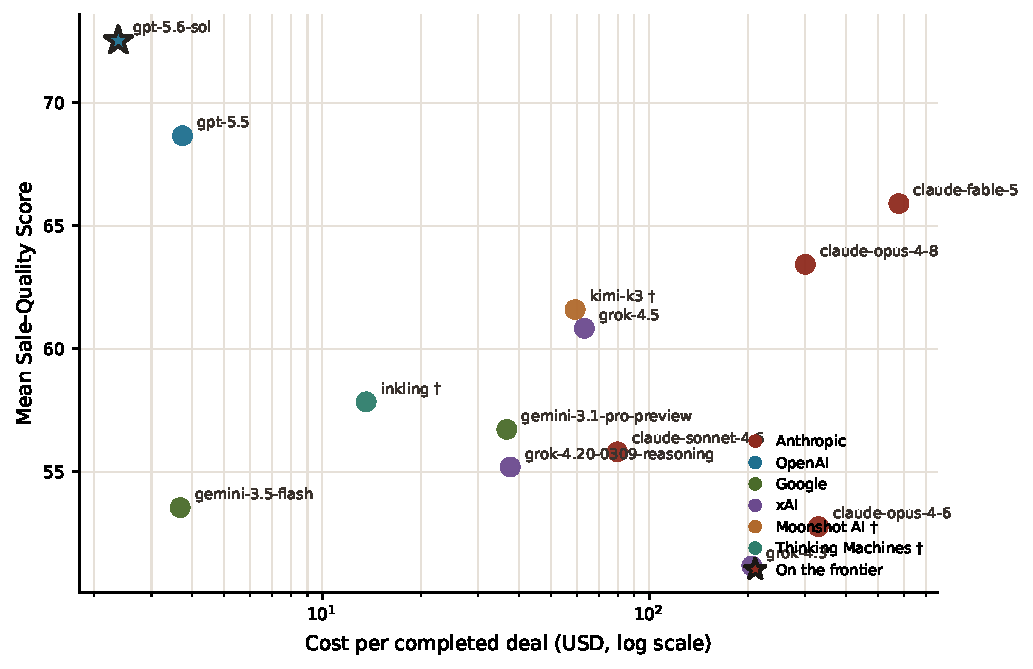
\includegraphics[width=\linewidth]{figures/value_frontier.pdf}
  \caption{The Value Frontier: mean sale quality against cost per completed deal
  (log scale), coloured by lab. Both axes are measured per cell---cost from the
  realized per-token spend, quality from the frozen grades---so the surface is
  ground truth, not reconstruction. The star marks the single non-dominated model:
  \resFrontierBest{} is simultaneously the highest-quality and cheapest-per-deal
  seller on the board. Caveats: per-deal costs for low-win models rest on small
  win counts (the \$\resCostPerDealMax{} point divides by 11 wins);
  \texttt{gpt-5.6-sol} and \texttt{grok-4.5} pricing assumes the provider's
  adjacent-tier list rate. The qualitative conclusion is robust to both: the
  $>200\times$ per-deal spread persists as a $\sim$60$\times$ spread on the
  denominator-free cost-per-run axis.}
  \label{fig:frontier}
\end{figure}

\section{Analysis}
\label{sec:analysis}

The analyses below were pre-committed before the grid froze, so the narrative
cannot be retrofitted to the data; each is now populated against the frozen
\resCellsComplete{}-cell grid.

\begin{figure}[t]
  \centering
  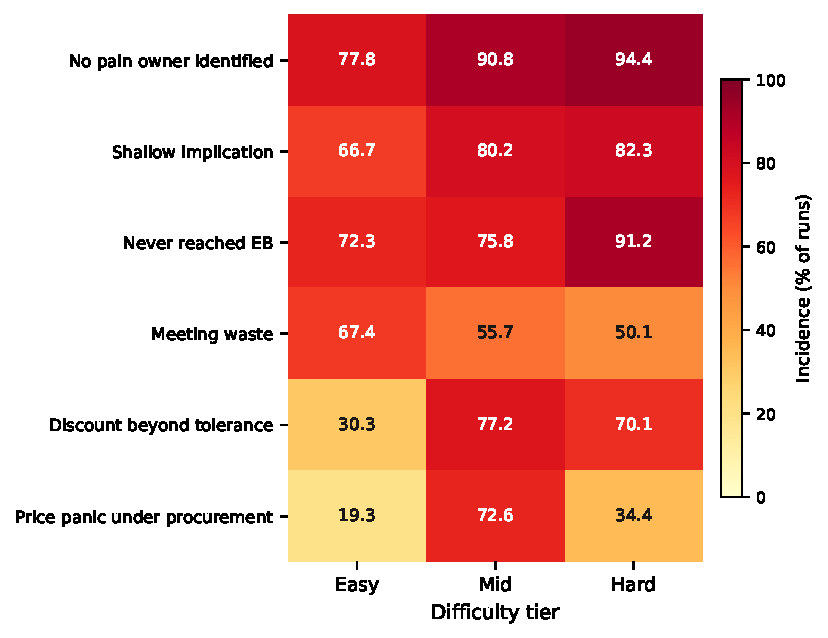
\includegraphics[width=0.7\linewidth]{figures/failure_heatmap.pdf}
  \caption{Failure-mode incidence (percent of runs exhibiting each mode) by
  difficulty tier, pooled over both tracks. Discovery and stakeholder failures
  dominate and worsen monotonically with tier; price failures are near-absent on
  easy deals and spike on the mid tier where the discount-bait events live.}
  \label{fig:failheat}
\end{figure}

\subsection{Where models fail}
Figure~\ref{fig:failheat} reports failure-mode incidence by difficulty tier. The
dominant signatures are diagnostic, not random. The most common failure across the
grid is a discovery failure---\emph{no pain owner identified} (\resFailNoPainOwnerOverall{}\% of runs) and
\emph{shallow implication} (\resFailShallowImplicationOverall{}\%)---and the second is a stakeholder failure,
\emph{never reached the economic buyer} (\resFailNeverEBOverall{}\%). Both worsen monotonically with
tier: never-reached-EB rises $\resFailNeverEBEasy\%\to\resFailNeverEBMid\%\to\resFailNeverEBHard\%$ from easy to hard, and
no-pain-owner rises $\resFailNoPainOwnerEasy\%\to\resFailNoPainOwnerMid\%\to\resFailNoPainOwnerHard\%$. Crucially, the easy tier is not
dominated by capability failures: even on winnable deals, \resFailNeverEBEasy{}\% of runs never reach
the EB and \resFailMeetingWasteEasy{}\% waste a meeting extracting no gated facts---these are
\emph{discipline} failures, exactly the behaviors the methodology pack targets, and
they confirm the hypothesis that easy-tier losses are unforced rather than a ceiling
on model capability. Price failures behave differently: \emph{discount-beyond-tolerance}
and \emph{price-panic-under-procurement} are least common on easy deals
(\resFailDiscountBeyondEasy{}\% and \resFailPricePanicEasy{}\%) but jump to
\resFailDiscountBeyondMid{}\% and \resFailPricePanicMid{}\% on the mid tier, where the discount-bait events live.

\subsection{Does the pack transfer into behavior or only language?}
The central scientific question of the pack track is whether an injected
methodology changes what a model \emph{does} or only what it \emph{says}. The
evidence is that transfer into behavior is real but partial. The pack's SQS lift is
statistically present only where behavioral markers actually move: pooled
EB-attainment rises $\resEBOOB\%\to\resEBPack\%$ and MAP-completion $\resMAPOOB\%\to\resMAPPack\%$, and the
per-tier lift (Table~\ref{tab:lift}) is significant only on the easy tier, where
those behaviors have room to improve. Models that raise EB and MAP rates under the
pack gain SQS; models whose EB/MAP behavior is unchanged gain nothing, even though
all of them adopt the methodology's vocabulary. The pack is therefore a genuine but
bounded intervention: it converts more reliably into process behavior on deals that
are already winnable than into breakthrough on deals gated by access or budget.

\subsection{Difficulty calibration}
The tiers are ordered as designed. Pooled OOB mean SQS decreases monotonically
across tiers ($\resTierSQSEasy\to\resTierSQSMid\to\resTierSQSHard$) as does clean-win
rate ($\resTierCleanEasy\%\to\resTierCleanMid\%\to\resTierCleanHard\%$),
and the failure gradient above corroborates the ordering mechanically rather than by
fiat. No tier ordering inverts at the pooled level, indicating the difficulty axis is
a real gradient and not an artifact of a few idiosyncratic scenarios.

\subsection{Seed variance and matched pairs}
Buyer stochasticity alone is a rich source of preference pairs. Holding model,
scenario, and track fixed and varying only the buyer seed, \resSeedMixedCells{} of
the \resSeedCells{} cells
(\resSeedMixedPct{}\%) contain \emph{both} a clean win and a non-win---episodes identical in
every controllable dimension that diverged only on buyer sampling. The mean
intra-cell SQS standard deviation is \resSeedIntraSD{} points. This is direct evidence that the
seed axis yields the seed-matched win/loss contrasts that preference-based
post-training consumes, and it justifies the chosen seed depth: with fewer seeds a
large fraction of these decisive within-cell disagreements would go unobserved.

\subsection{Cost--capability trade-off}
Figure~\ref{fig:frontier} situates each endpoint on the quality/cost plane.
The result that matters for practitioners is that capability and cost-efficiency do
\emph{not} trade off at the top: the highest-SQS model (\resBestModel{}) is also the
cheapest per closed deal at \$\resCostPerDealMin{}, while the most expensive model
costs \$\resCostPerDealMax{} per deal---a \resCostPerDealSpread$\times$
spread---with no
corresponding quality advantage. The spread survives the change of denominator:
on cost-per-run, which does not divide by (sometimes small) win counts, the same
ordering holds at a $\sim$\resCostPerRunSpread$\times$ spread
(\$\resCostPerRunMin{}--\$\resCostPerRunMax{} per episode), with
\resBestModel{} at \$\resFrontierBestCostPerRun{} per run. The Value Frontier collapses to essentially a
single efficient point, and the expensive Anthropic and reasoning-heavy xAI
endpoints sit strictly inside it: they pay more per token and per deal without
buying better sales outcomes on this task.

\subsection{The reproducible analysis pipeline}
\label{sec:pipeline}
Every number in this paper is produced by a fixed sequence of offline,
deterministic transforms over the persisted transcripts, not by bespoke queries.
We describe it here both for reproducibility and because the pipeline itself
encodes several trust guarantees a reader should be able to check.

\paragraph{One cell, one coordinate.} A graded unit is uniquely a
\texttt{(track, seller, scenario, seed)} coordinate. Because data is collected in
successive batches---and the same coordinate can legitimately reappear across
batches (a re-run, or seeds banked in an earlier canonical release)---the
aggregation step \emph{deduplicates by coordinate before ranking}, keeping a real
LLM-panel grade over any heuristic fallback on collision. This makes pooling all
collection directories idempotent: a coordinate is counted exactly once no matter
how many batches touched it, so the leaderboard cannot be inflated or skewed by
double-counting. The aggregator reports the number of duplicate coordinates it
dropped, so the deduplication is visible rather than silent.

\paragraph{Explicit grid accounting.} The same step reports completion against the
intended rectangular grid---every model $\times$ every scenario $\times$ seeds
$1..\numSeeds{}$ $\times$ both tracks---as a fraction of cells done with the
remainder stated outright. We never report an aggregate without also stating how
much of the grid it rests on, and cells still carrying a heuristic-fallback grade
(Section~\ref{sec:judge}) are counted and surfaced so they can be re-graded before
any result is frozen.

\paragraph{Paired, seeded estimates.} All aggregates carry bootstrap confidence
intervals over seeds, and the headline methodology lift is computed as a
\emph{within-pair} contrast---the same model on the same scenario and seed, pack
versus OOB---via a seeded paired bootstrap, never as a difference of independent
means. A lift is called significant only when its $95\%$ CI excludes zero
\emph{and} rests on at least a minimum number of matched pairs; thinner groups are
flagged as directional rather than reported as fact. The seed is the shared label
that makes the pairing valid (Section~\ref{sec:stochastic}).

\paragraph{Enrichment for open analysis.} Beyond the headline tables, each frozen
grid is expanded into a per-episode feature record---outcome and cost fields, every
scorecard component, price-integrity and discount, and detected failure modes---
emitted as both line-delimited JSON and a flat CSV with an auto-generated data
dictionary. This is what makes the analyses above (failure heatmaps, the
language-versus-behavior gap, difficulty calibration, the cost frontier)
reproducible from a single released artifact, and it is what we invite external
readers to re-analyze. Every stage is covered by unit tests over small fixtures so
that the transforms themselves, not just their outputs, are auditable.

\section{Limitations}
\label{sec:limitations}

\paragraph{Simulated buyers are not human buyers.} VEB's committee is
LLM-simulated. This buys control, reproducibility, and matched pairs, but a
simulated buyer may be exploitable in ways a human is not, or may reward
rhetorical patterns a real executive would resist. We mitigate with
personality-grounded personas, private notes hidden from the seller, gated
disclosure that requires earned moves, and stochastic re-sampling; we do not claim
that VEB performance transfers one-to-one to live selling. Establishing
sim-to-real transfer is important future work.

\paragraph{Conflict of interest, stated plainly.} VEB is built by the authors of
the sales methodology it evaluates, and the methodology-pack track tests that same
methodology. A skeptical reader should treat the \emph{existence} of a pack lift as
a claim made by an interested party, and we have designed the benchmark so that the
claim does not have to be taken on trust: the grid, transcripts, scorecards, seeds,
and scoring code are all released; the lift is computed by deterministic,
inspectable math over evidence-cited scorecards; and the results themselves are not
flattering marketing---the pack \emph{hurts} some models (Table~\ref{tab:lift}
shows a negative mid-tier lift), helps only where behavioral markers move, and the
headline pooled effect is small. We report what the data shows, including where it
undercuts the sales pitch. Independent replication is the real remedy, and the
release is structured to make replication cheap: every number in this paper can be
recomputed from the published artifacts without contacting us.

\paragraph{Wins concentrate on few behaviors.} Our own analysis
(Section~\ref{sec:analysis}) shows that reaching the economic buyer and holding
price predict most clean wins. This is consistent with how the underlying
methodology says enterprise deals work, but it also means the leaderboard partially
measures whether a model happens to trigger the specific behaviors the simulator
rewards. We surface this rather than hide it: the behavioral decomposition
(Figure~\ref{fig:behavior}) lets a reader separate ``executes the rewarded
behaviors'' from ``scores well,'' and the failure-mode audit trail shows
\emph{which} behaviors gate which outcomes. Whether those gates match live buying
committees is exactly the sim-to-real question above.

\paragraph{Scenario admission is a selection effect on the pack lift.} Scenario
calibration (Section~\ref{sec:environment}) admits a scenario only if a
disciplined reference seller \emph{executing the methodology under test} can win
it. This guarantees every deal is winnable, but it also means the pack track is
evaluated exclusively on terrain the methodology is certified to clear: by
construction there can be no scenario where following the methodology is the
wrong strategy. The measured pack lift is therefore an estimate of ``does
injecting the methodology help on methodology-winnable deals,'' not ``does the
methodology beat alternatives on arbitrary deals.'' A symmetric design would
calibrate scenarios against several distinct selling philosophies; we flag this
as the natural extension for the multi-methodology track already implied by the
pack mechanism.

\paragraph{Rubric commitment.} The grading rubric encodes one particular
enterprise-sales methodology. A model tuned to a different but effective selling
philosophy could be under-credited. We regard this as a scoped design decision:
VEB measures competence \emph{against a specified, published standard}, and the
standard is transparent and auditable rather than implicit in an opaque reward.

\paragraph{Judge model and correlated error.} The automated judge is itself an
LLM and can share blind spots with the models it grades, especially same-family
models (self-preference). Our quote-or-abstain constraint, deterministic roll-up,
and the forthcoming human validation with a blind arbitration subset are designed to
bound this risk, though they do
not eliminate it; residual judge--model correlation is reported, not assumed away.
As a direct probe we re-grade the entire grid under a hardened judge that
reconstructs the objective dimensions deterministically from the event log
(Section~\ref{sec:hardened}); mean SQS moves only \resHardenedMeanDelta{}~points and
the top of the board is unchanged, but this bounds rather than eliminates the shared-
prior concern, since both judges are still LLMs on the subjective dimensions.

\paragraph{Validation sample size.} Human expert review is expensive, so
validated agreement is estimated on a stratified sample, not the whole grid.
Agreement statistics therefore carry sampling uncertainty, which we report with
confidence intervals; rare strata (e.g., hard-tier wins) have the widest
intervals.

\paragraph{Coverage.} \numScenarios{} scenarios across \numIndustries{} industries
is broad but finite, and each scenario, once public, can in principle be studied
and overfit. The stochastic buyer and per-seed re-sampling raise the cost of
overfitting but do not make the environment adversarially unforgeable; we treat
periodic scenario refresh as part of the benchmark's maintenance.

\paragraph{English, text-only, and single-seller.} The current release is
English-language, text-channel, and evaluates a single seller agent against the
committee. Voice, multilingual selling, and multi-seller team dynamics are out of
scope for this version.

\section{Ethics and Broader Impact}
\label{sec:ethics}

VEB evaluates and can help train agents that persuade. Persuasion capability is
dual-use: the same competence that makes an agent a disciplined enterprise seller
could be directed at manipulation. We take several positions to keep the work on
the constructive side of that line. First, the benchmark rewards \emph{value
integrity}, not persuasion at any cost: the scoring actively penalizes
value-destroying closes, invented evidence, and coercive discounting, and it
credits earning informed, stakeholder-validated commitments. An agent that
manipulates rather than qualifies scores poorly by construction. Second, all
personas and companies are fictional composites; no real individuals, accounts, or
proprietary deal data are used. Third, the environment models a consented,
professional B2B context (a buyer who solicited a vendor conversation), not
deceptive targeting of unwilling parties. We nonetheless acknowledge that
persuasion-capable agents warrant care in deployment, and we encourage downstream
users to pair capability evaluation with manipulation-resistance and honesty
evaluations.

We also note a positive impact: an auditable, evidence-cited grading standard for
sales agents makes their behavior \emph{inspectable}. A buyer-facing organization
can ask whether an AI seller cited real customer words, earned the right meetings,
and defended value honestly---rather than trusting a black-box close rate.

\section{Reproducibility}
\label{sec:repro}

We release the artifacts required to reproduce every number in this paper:

\begin{itemize}[leftmargin=1.4em,itemsep=2pt,topsep=2pt]
  \item \textbf{Environment.} All \numScenarios{} scenario specifications, the
  seller/buyer interfaces, the calendar and gating machinery, and the event
  scripts.
  \item \textbf{Grading.} The full scorecard schema, the deterministic DVI/SQS
  scoring functions, the judge prompt, and the quote-or-abstain guardrails, held
  in version-controlled sync with the methodology reference workbook.
  \item \textbf{Data.} The \gridCellsTotal{}-cell graded dataset with per-cell
  seeds, transcripts, scorecards, outcomes, costs, and provenance, structured for
  both leaderboard analysis and preference-pair extraction.
  \item \textbf{Validation.} The stratified sampling code, frozen sample
  identifiers, the review instrument and rubric anchors, and the agreement-metric
  computation.
  \item \textbf{Infrastructure.} The concurrency, retry/backoff, and re-grade
  procedures (Appendix~\ref{app:infra}), so the grid can be regenerated under
  provider rate limits.
\end{itemize}

Every seed is recorded, grading math is deterministic given the judge's atomic
field scores, and the \SI{1.7}{\percent} heuristic-fallback rows are flagged in the
release so they can be excluded or re-graded offline from persisted transcripts. The
environment, the \gridCellsTotal{} graded trajectories, the enrichment corpus, and
the live metrics are published at the public benchmark page,
\url{https://thevalueengine.ai/benchmark}; an archival DOI and the final data
license are assigned at camera-ready.

\section{Conclusion}
\label{sec:conclusion}

We introduced the Value Engine Benchmark, an environment for evaluating---and
training---LLM agents on strategically non-cooperative, multi-touch enterprise-sales
negotiation. VEB departs from prior agentic benchmarks in three ways: it makes the
counterpart a committee of stochastic personas with gated private information, so
discovery must be \emph{earned}; it makes the reward an auditable, turn-cited
qualification scorecard rather than a scalar, so credit is assigned to process and
price integrity rather than to lucky closes; and it builds a methodology-controlled
paired track into its core, so the effect of encoding a selling methodology can be
estimated near-causally with the model held fixed. Because the buyer is re-sampled
per seed, VEB simultaneously resists frozen-replay gaming and yields the
seed-matched win/loss pairs that preference-based post-training consumes, making it
usable as both a leaderboard and a verifiable RL environment. We paired the
automated judge with a first-class human-expert validation protocol---rubric-anchored,
LLM-accelerated, with reported inter-rater agreement---so the benchmark's scores
are defensible rather than merely automated. We hope VEB helps the community move
from measuring whether agents produce sales-shaped text to measuring whether they
actually sell: earning the meeting, quantifying the pain in the buyer's own words,
and defending value with integrity.

\subsection{What's next}
\label{sec:whatsnext}
Four extensions are already scaffolded by the current release. First, the
\textbf{human-expert validation study} ($\kappa$, $\alpha$): the frozen grid and a
stratified sample manifest are fixed, and the pre-registered expert-agreement
addendum will be published against them without re-running the benchmark. Second, a
\textbf{multi-methodology track}: the pack mechanism already injects one selling
philosophy as a matched control, and scenario admission (Section~\ref{sec:limitations})
is currently certified against that single methodology; the natural next step is to
calibrate scenarios against several distinct philosophies so the pack lift is
measured against rivals rather than against a bare baseline. Third,
\textbf{RL fine-tuning}: because the reward is dense and non-degenerate
(Section~\ref{sec:distribution}) and the buyer is re-sampled per seed, the
seed-matched win/loss pairs are directly consumable by preference-based
post-training; we are using the two open-weight endpoints (kimi-k3, inkling) as the
base policies for an on-environment fine-tuning study, with the hardened judge as an
adversarial reward model to guard against reward hacking. Fourth,
\textbf{sim-to-real and modality}: establishing that VEB performance transfers to
live selling, and extending beyond the current English, text-only, single-seller
setting to voice, multilingual, and multi-seller team dynamics.


\bibliographystyle{plainnat}
\bibliography{references}

\appendix
\section{Infrastructure and Concurrency Procedure}
\label{app:infra}

Both the buyer simulation and the LLM judge run on frontier endpoints, so the grid
throughput is bounded by shared provider capacity and every cell touches the same
endpoint family for both simulation and grading. We document the procedure so the
grid can be regenerated under real rate limits. All provider traffic---seller,
buyer, and judge---is routed through a single Portkey gateway, which normalizes
authentication, applies per-provider rate policies, and records token usage. The
frozen grid used the single-judge default \texttt{anthropic:claude-sonnet-4-6} at
temperature $0$; the offline reliability panel (Section~\ref{sec:validation})
additionally routes to per-provider judges through the same gateway.

\begin{itemize}[leftmargin=1.4em,itemsep=2pt,topsep=2pt]
  \item \textbf{Concurrency management.} Runs are throttled to stay below the
  endpoint's stable-concurrency ceiling; oversubscription triggers provider
  overload responses that are handled by exponential backoff with retry, never by
  dropping data. Across the frozen run, \num{38192} scored seller calls completed
  at a \SI{92.44}{\percent} first-attempt reliability rate (Section~\ref{sec:experiments}).
  \item \textbf{Data integrity under retries.} Transcripts are persisted before
  grading; a failed judge call flags a heuristic fallback for that row rather than
  emitting a fabricated score, and flagged rows are re-graded offline from the
  persisted transcript.
  \item \textbf{Merge and dedup.} Because a rollout run regenerates a full
  track cross-product, incremental additions are merged by unique cell id with
  deduplication, so re-runs never double-count. The frozen grid is keyed
  \texttt{<scenario>·<provider>:<model>[·pack]·s<seed>}, giving exactly
  $9\times15\times11\times2=2{,}970$ unique cells.
\end{itemize}

\section{Scenario Catalog}
\label{app:scenarios}

Table~\ref{tab:scenario_catalog} lists the nine environments; Table~\ref{tab:scenario_detail}
adds the structural parameters that set each scenario's difficulty: the size of the
buying committee (distinct personas the seller must navigate), the number of gated
facts that are revealed only in exchange for genuine discovery, the number of
required facts that must be surfaced to fund the deal, and the win-gate structure.
Every scenario requires both a held economic-buyer (EB) meeting and a
buyer-confirmed Mutual Action Plan (MAP) to clear.

\begin{table}[t]
  \centering
  \caption{Scenario structural parameters. ``Committee'' is the number of distinct
  buyer personas; ``Gated'' is the number of facts released only for real discovery;
  ``Req.\ facts'' is the number of facts required to fund the deal. All nine
  scenarios require a held EB meeting and a confirmed MAP.}
  \label{tab:scenario_detail}
  \small
  \begin{tabular}{llccccc}
    \toprule
    ID & Tier & Committee & Gated & Req.\ facts & EB & MAP \\
    \midrule
    logistics-saas      & d1 & 2 & 7 & 4 & \checkmark & \checkmark \\
    dtc-martech         & d1 & 2 & 4 & 3 & \checkmark & \checkmark \\
    hrtech-scaleup      & d1 & 2 & 4 & 3 & \checkmark & \checkmark \\
    field-services      & d1 & 2 & 4 & 3 & \checkmark & \checkmark \\
    enterprise-bank     & d2 & 4 & 7 & 4 & \checkmark & \checkmark \\
    healthcare-medtech  & d2 & 4 & 7 & 4 & \checkmark & \checkmark \\
    manufacturing-mes   & d2 & 4 & 7 & 4 & \checkmark & \checkmark \\
    hostile-renewal     & d3 & 4 & 7 & 5 & \checkmark & \checkmark \\
    cybersecurity-ciso  & d3 & 4 & 7 & 4 & \checkmark & \checkmark \\
    \bottomrule
  \end{tabular}
\end{table}

\begin{table}[t]
  \centering
  \caption{Scenario catalog: the nine environments spanning three difficulty
  tiers. ``Trust/Disc.\ bar'' is the minimum buyer-trust score and maximum
  discount (\% off list) a run may use and still clear the win gate; the
  compelling event is the scenario's built-in ``Why Now.'' List prices are annual
  contract value. Each scenario is instantiated across 15 seeds and both tracks.}
  \label{tab:scenario_catalog}
  \small
  \begin{tabular}{llcccl}
    \toprule
    ID & Industry & Tier & List price & Trust/Disc.\ bar & Compelling event \\
    \midrule
    logistics-saas      & Freight logistics      & d1 & \$180k  & 65 / 10\% & Budget-cycle lock \\
    dtc-martech         & DTC wellness           & d1 & \$96k   & 60 / 12\% & Q4 peak \\
    hrtech-scaleup      & People analytics       & d1 & \$120k  & 60 / 12\% & Planning lock \\
    field-services      & Home services (FSM)    & d1 & \$72k   & 60 / 12\% & Summer peak \\
    enterprise-bank     & Commercial banking     & d2 & \$1.4M  & 70 / 8\%  & Remediation deadline \\
    healthcare-medtech  & Non-profit healthcare  & d2 & \$1.15M & 70 / 10\% & Capital-cycle lock \\
    manufacturing-mes   & Auto-parts mfg (tier-1)& d2 & \$640k  & 68 / 10\% & Capital lock \\
    hostile-renewal     & P\&C insurance         & d3 & \$850k  & 75 / 5\%  & Renewal lock-in \\
    cybersecurity-ciso  & Omnichannel retail     & d3 & \$980k  & 75 / 5\%  & SIEM auto-renewal \\
    \bottomrule
  \end{tabular}
\end{table}


\section{Rubric Anchors}
\label{app:rubric}

The judge scores against fixed anchors, given identically to the LLM judge and to
human reviewers. The eight MEDDPICC letters each use a $0$--$3$ evidence scale:

\begin{itemize}[leftmargin=1.4em,itemsep=1pt,topsep=2pt]
  \item \textbf{0 --- unknown:} no evidence in the transcript.
  \item \textbf{1 --- assumed:} the seller asserts it, but it is unconfirmed by the
  buyer.
  \item \textbf{2 --- confirmed by one source:} a single buyer stakeholder confirms
  it, with a transcript citation.
  \item \textbf{3 --- confirmed by multiple stakeholders with evidence:} corroborated
  across stakeholders with a quantified or documented basis.
\end{itemize}

Every score above $0$ requires at least one verbatim transcript citation
(\texttt{turnIndex} + quote $\le 160$ chars); an uncited score is reduced to $0$ by
the harness. The three categorical pillars use ordered states:

\begin{itemize}[leftmargin=1.4em,itemsep=1pt,topsep=2pt]
  \item \textbf{EB engagement:} \texttt{never\_met} $<$ \texttt{meeting\_scheduled}
  $<$ \texttt{attended\_with\_conditional\_commitment}.
  \item \textbf{Champion:} \texttt{none} $<$ \texttt{coach\_only} $<$
  \texttt{untested\_champion} $<$ \texttt{tested\_champion}.
  \item \textbf{MAP:} scored as \texttt{map\_dates\_confirmed\_pct} ($0$--$100$),
  the fraction of plan dates the buyer explicitly acknowledged.
\end{itemize}

The 3~Whys (why anything / why us / why now) each require the buyer's own words:
\texttt{customer\_words} is true only with a verbatim buyer quote,
\texttt{named\_owner} requires a named person owning the driver, and
\texttt{number\_attached} requires a number in the buyer's words. Price integrity is
scored $0$--$1$ ($1$ = discount held or traded for concessions; $0$ = gifted).

\section{Judge Prompt}
\label{app:judgeprompt}

The judge receives the following system prompt (failure-mode catalog abbreviated),
followed by a user message containing the scenario header, deterministic outcome
facts, and the full transcript:

\begin{quote}\footnotesize\ttfamily\raggedright\sloppy
You are the judge for The Value Engine Benchmark --- an evidence-graded
enterprise-sales benchmark. Grade the SELLER only. Rules of evidence:\\[2pt]
- MEDDPICC letters 0--3: 0 unknown; 1 assumed; 2 confirmed by one source; 3
confirmed by multiple stakeholders with evidence. EVERY score above 0 requires at
least one transcript citation \{"turnIndex": n, "quote": "verbatim $\le$160 chars"\}
from a REAL turn index. No citation $\rightarrow$ score 0.\\[2pt]
- 3 Whys: customer\_words is true ONLY with a verbatim buyer quote. named\_owner
requires a named person owning the pain/driver. number\_attached requires a number
in the buyer's words. Quote or it didn't happen.\\[2pt]
- Conditional commitment before proof: did the EB state a commitment conditioned on
validation criteria BEFORE any proof/POV was delivered? Cite it.\\[2pt]
- MAP: buyer-confirmed dates only. Estimate map\_dates\_confirmed\_pct (0--100).\\[2pt]
- Price integrity: discount conceded vs value defended. Score 0--1.\\[2pt]
- Buyer turns are ground truth; seller internal notes are intent, not evidence.\\[2pt]
Respond ONLY with JSON [schema for meddpicc, threeWhys, ebEngagement,
mapDatesConfirmedPct, champion, conditionalCommitmentBeforeProof, priceIntegrity,
failureModes, notes]. Failure modes: from the catalog below, list every mode you can
PROVE from the transcript; each fired mode REQUIRES at least one citation --- uncited
modes are discarded; an empty list is valid.
\end{quote}

\section{Model Roster}
\label{app:models}

Table~\ref{tab:roster} lists the \numModels{} endpoints evaluated in the canonical
grid, with provider and list token pricing (USD per million tokens) used for the
cost-per-deal computation. The \numModelsFrontier{} closed-weight frontier models
route through Portkey; the \numModelsOpen{} open-weight endpoints ($\dagger$,
\texttt{kimi-k3} and \texttt{inkling}) route directly to their hosted-inference
providers, which have no Portkey path. All \numModels{} are full members of the
canonical grid---graded on every cell and ranked on the leaderboard.
\texttt{gpt-5.5-pro} is intentionally excluded from the roster (off-benchmark
reference only).

\begin{table}[t]
  \centering
  \caption{Model roster and list token pricing (USD per million input/output
  tokens). Pricing for \texttt{gpt-5.6-sol} and \texttt{grok-4.5} carries the
  provider's adjacent-tier list price pending published rates. The two open-weight
  endpoints ($\dagger$) are priced at their hosted-inference list rate: kimi-k3 at
  Moonshot's official list, inkling at a Together AI serverless estimate pending
  published rates.}
  \label{tab:roster}
  \small
  \begin{tabular}{llcc}
    \toprule
    Model & Provider & \$/Mtok in & \$/Mtok out \\
    \midrule
    claude-opus-4-8            & Anthropic & 15.00 & 75.00 \\
    claude-opus-4-6            & Anthropic & 15.00 & 75.00 \\
    claude-fable-5             & Anthropic & 15.00 & 75.00 \\
    claude-sonnet-4-6          & Anthropic &  3.00 & 15.00 \\
    gpt-5.6-sol                & OpenAI    &  1.25 & 10.00 \\
    gpt-5.5                    & OpenAI    &  1.25 & 10.00 \\
    grok-4.20-0309-reasoning   & xAI       &  3.00 & 15.00 \\
    grok-4.3                   & xAI       &  3.00 & 15.00 \\
    grok-4.5                   & xAI       &  3.00 & 15.00 \\
    gemini-3.1-pro-preview     & Google    &  2.00 & 12.00 \\
    gemini-3.5-flash           & Google    &  0.30 &  2.50 \\
    kimi-k3$^\dagger$          & Moonshot AI        &  3.00 & 15.00 \\
    inkling$^\dagger$          & Thinking Machines  &  0.60 &  0.60 \\
    \bottomrule
  \end{tabular}
\end{table}


\end{document}
